%\setcounter{chapter}{36}

\chapter{Transfer Learning and Adaptation}
\label{chapter:transfer_learning}

\section{Introduction}

A common criticism of deep learning systems is that they are data hungry. To learn a new concept (e.g., ``is this a dog?'') may require showing a deep net thousands of labeled examples of that concept. Conversely, humans can learn to recognize a new kind of animal after seeing it just once, an ability known as \index{One-shot learning}{\bf one-shot learning}.\marginnote{Correspondingly, \index{Few-shot learning}\textbf{few-shot learning} refers to learning from just a few examples, and the \textbf{zero-shot} setting refers to when a model works out of the box on a new problem, with zero adaptation whatsoever.}[-0.0cm]

Humans can do this because we have extensive prior knowledge we bring to bear to accelerate the learning of new concepts. Deep nets are data hungry when they are trained from \emph{scratch}. But they can actually be rather data efficient if we give them appropriate prior knowledge and the means to use their priors to accelerate learning. Transfer learning deals with how to use prior knowledge to solve new learning problems quickly.

Transfer learning is an alternative to the ideas we saw last chapter, where we simply trained on a broad distribution of data so that most test queries happen to be things we have encountered before. Because it is usually impossible to train on \textit{all} queries we might encounter, we often need to rely on transfer learning to adapt to new kinds of queries.

%especially valuable for handling the problem out of distribution generalization, which we encountered in the last chapter. We need ways to adapt our model gracefully when the world changes or when our goals change.

\section{Problem Setting}

Suppose you are working at a farm and the drones that water the plants need to be able to recognize whether the crop is wheat or corn. Using the machinery we have learned so far, you know what to do: gather a big dataset of aerial photos of the crops and label each as either wheat or corn, then, train your favorite classifier to perform the mapping $f_{\theta}: \mathcal{X} \rightarrow \{\texttt{wheat}, \texttt{corn}\}$. It works! The crop yield is plentiful. Now a new season rolls around and it turns out the value of corn has plummeted. You decide to plant soybeans instead. So, you need a new classifier; what should you do?

One option is to train a new classifier from scratch, this time on images of either wheat or soybeans. But you already know how to recognize wheat; you still have last year's classifier $f_{\theta}$. We would like to make use of $f_{\theta}$ to accelerate the learning of this year's new classifier. Transfer learning is the study of how to do this. 

Transfer learning algorithms involve two parts:
\begin{enumerate}
    \item \index{Pretraining}\textbf{Pretraining}: how to acquire prior knowledge in the first place.
    \item \textbf{Adaptation}: how to use prior knowledge to solve a new task.
\end{enumerate}

In our example, the pretraining phase was training the wheat versus corn classifier, and the adaptation phase is updating that classifier to instead recognize wheat versus soybeans. This is visualized below in \fig{\ref{fig:transfer_learning:finetuning_basic}}.%\marginnote{By convention, we call the first phase of training ``pretraining" and the second stage ``finetuning", since often pretraining involves extensive training ``in the factory", on a big dataset and thousands of processors, whereas usually finetuning refers to small updates done ``in the wild" or on-device, with far fewer computational and data resources.}[-0.83cm]
\begin{figure}[h!]
    \centering
    \centerline{
    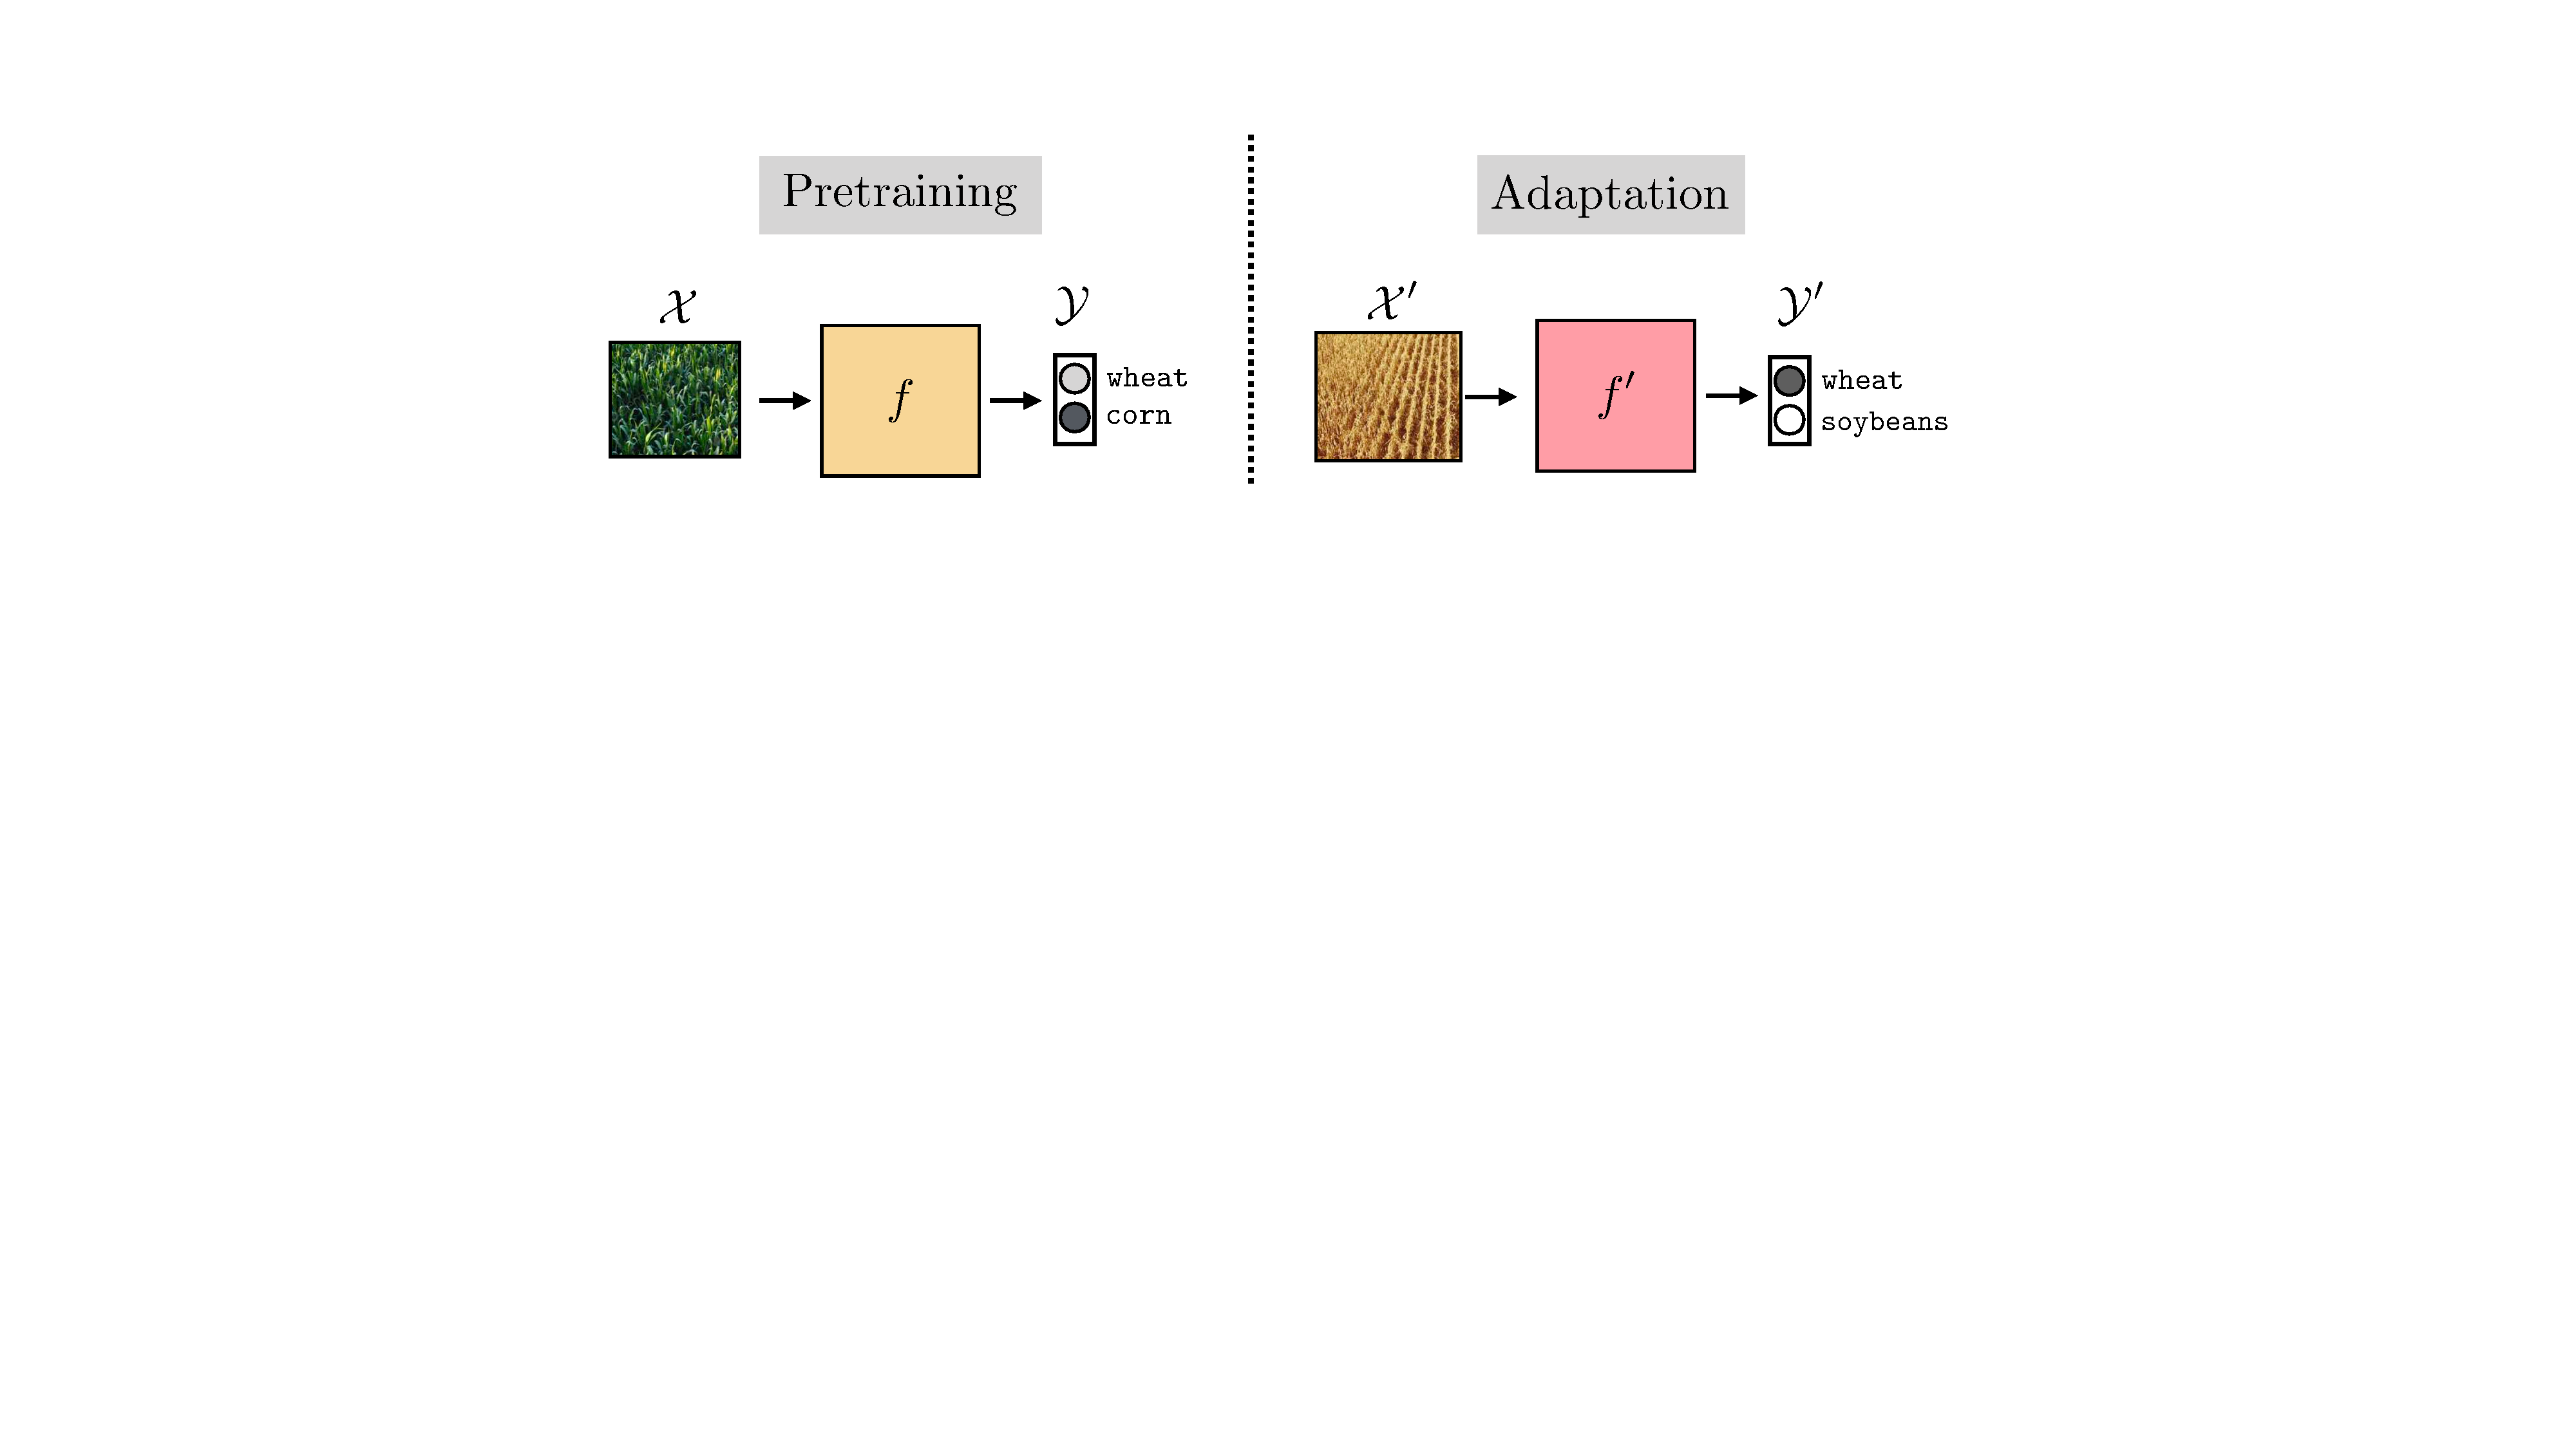
\includegraphics[width=0.85\linewidth]{./figures/transfer_learning/pretraining_and_adaptation.pdf}
    }
    \caption{Transfer learning consists of two phases: first we pretrain a model on one task and then we adapt that model to perform a new task.}
    \label{fig:transfer_learning:finetuning_basic}
\end{figure}

\marginnote{The pretraining phase could just be regular training, which we only call \textit{pre}training in retrospect, once we decide to start adapting to a new problem. Or we can specifically design pretraining algorithms that are \textit{only} meant as a warm up for the real event. Representation learning algorithms (\chap{\ref{chapter:representation_learning}}) are of this latter variety.}

In the next sections we will describe specific kinds of transfer learning algorithms, which handle each of these stages in different ways. Then, in \sect{\ref{sec:transfer_learning:combinatorial_catalog}}, we will reflect on the landscape of choices we have made, and we will see that transfer learning is better understood as a collection of tools, which can be combined in innumerable ways, rather than as a set of specific named algorithms.%\marginnote{In general, we feel that this is a more advanced way of looking at methods in computer vision. While it to sometimes convenient to give methods categorical names like ``finetuning" or ``prompting", it is more nuanced to see all these methods as part of a spectrum, with rich interrelationships and fuzzy boundaries.}


% \begin{table}[h]
%     \centering
%     \begin{tabular}{l|c|c}
%         Method & What is transferred & What is adapted \\
%         \hline
%         Prompting & Mapping & Inputs \\
%         Domain adaptation & Mapping & Inputs \\
%         Finetuning & Mapping init & Mapping \\
%         Distillation & Targets & Mapping \\
%         Linear probes & Mapping & Outputs
%     \end{tabular}
%     \caption{Different kinds of adaptation.}
%     \label{tab:transfer_learning:types_of_transfer_learning}
% \end{table}

\section{Finetuning}
\index{Finetuning}

There are many ways to do transfer learning. We will start with perhaps the simplest: when you encounter a new task, just keep on learning \emph{as if nothing happened}.

\textbf{Finetuning} consists of initialializing a new classifier with the parameter vector from the pretrained model, and then training it as usual. In other words, finetuning is making small (fine) adjustments (tuning) to the parameters of your model to adapt it to do something slightly different than what it did before, or even something a lot different.

There are three stages: (1) pretrain $f: \mathcal{X} \rightarrow \mathcal{Y}$, (2) initialize $f^{\prime} = f$, and (3) finetune $f^{\prime}: \mathcal{X}^{\prime} \rightarrow \mathcal{Y}^{\prime}$. The full algorithm is written in \algref{\ref{alg:transfer_learning:finetuning}}, with $f$ and $f^{\prime}$ indicated as just a continually learning $f_{\theta}$ with different iterates of $\theta$ as learning progresses.

\begin{algorithm}[h]
\SetAlgoVlined
\DontPrintSemicolon
%\marginnote{{\bf Algorithm \ref{alg:transfer_learning:finetuning}}: Using gradient descent to train one model and then finetuning to produce a second model.}
\caption{{\bf Algorithm \ref{alg:transfer_learning:finetuning}}: Finetuning. Using gradient descent to train one model and then finetuning to produce a second model.}
\fakealgorithmcaption{}
\label{alg:transfer_learning:finetuning}
{\bf Input:} initial parameter vector $\theta^{0}$, data $\{x^{(i)},y^{(i)}\}_{i=1}^N$, $\{x^{\prime^{(i)}},y^{\prime^{(i)}}\}_{i=1}^M$, learning rates $\eta_1$ and $\eta_2$\;
{\bf Output:} trained models $f_{\theta^{N}}$ and $f_{\theta^{N+M}}$\;
{\bf Pretraining:} \For{\upshape $k = 1, \dots, K_1$} {
    $J = \mathbb{E}_{x,y}[\mathcal{L}(f_{\theta^{k-1}}(x),y)]$\;
    $\theta^{k} \leftarrow \theta^{k-1} - \eta_1 \nabla_{\theta} J$\;
}
{\bf Finetuning:} \For{\upshape $k = 1, \dots, K_2$} {
    $J = \mathbb{E}_{x^{\prime},y^{\prime}}[\mathcal{L}(f_{\theta^{k-1+N}}(x^{\prime}),y^{\prime})]$\;
    $\theta^{k+N} \leftarrow \theta^{k-1+N} - \eta_2 \nabla_{\theta} J$\;
}
\end{algorithm}

Finetuning is simple and works well. But there is one tricky bit we still need to deal with: What if the structure of $f_{\theta}$ is incompatible with the new problem we wish to finetune on?

For example, suppose $f$ is a neural net and $\theta$ are the weights and biases of this net. Then the previous algorithm will only work if the dimensionality of $\mathcal{X}$ matches the dimensionality of $\mathcal{X}^{\prime}$, and the same for $\mathcal{Y}$ and $\mathcal{Y}^{\prime}$. This is because, for our neural net model, $f_{\theta}$ must have the same shape inputs and outputs regardless of the values $\theta$ takes on. What if we start with our net trained to classify between wheat and corn and now want to finetune it to classify between wheat, corn, and soybeans? The dimensionality of the output has changed from two classes to three.

To handle this it is common to cut off the last layer of the network and replace it with a new final layer that outputs the correct dimensionality. If the input dimensionality changes, you can do the same with the first layer of the network. Both these changes are shown next, in \fig{\ref{fig:transfer_learning:finetuning_stages}}. %Here's what this looks like:
\begin{figure}[h]
    \centerline{
    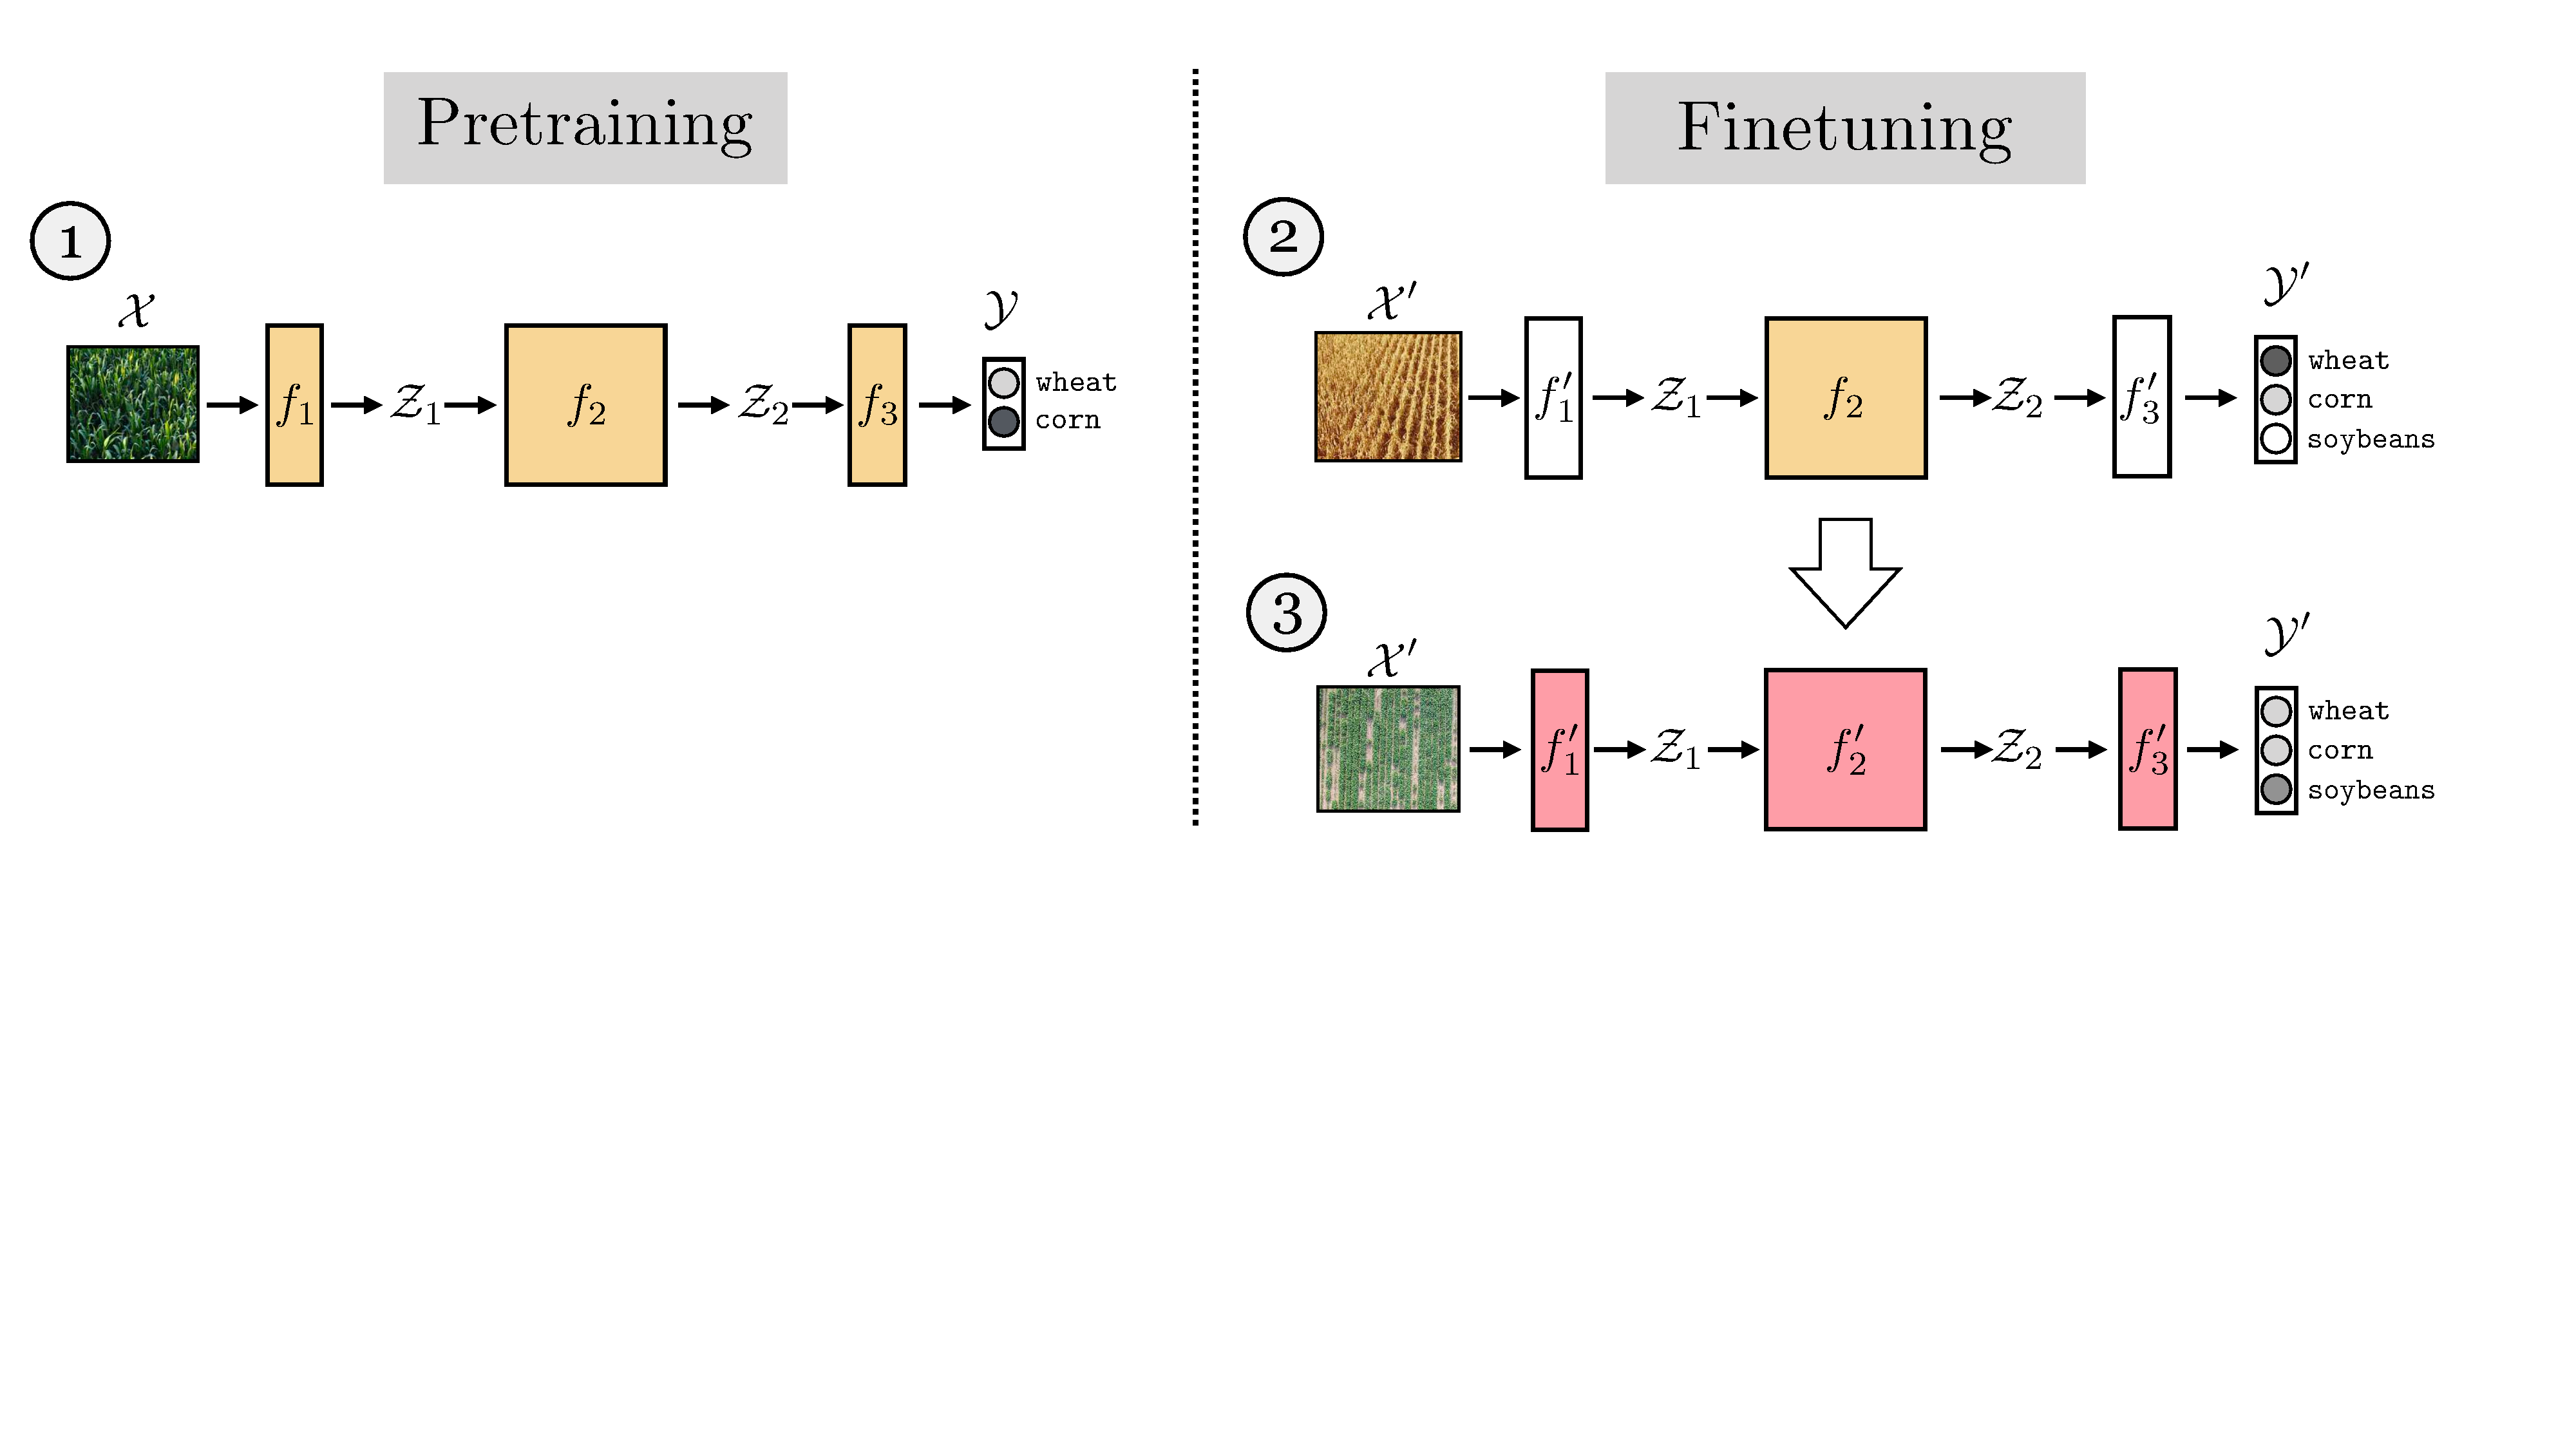
\includegraphics[width=1.0\linewidth]{./figures/transfer_learning/finetuning_stages.pdf}
    }
    \caption{Finetuning diagram.\\ \hfill \break
    \parbox[t]{0.32\textwidth}{
        \raisebox{-0.7mm}{\crule[pretrained_color_bright]{3mm}{3mm}} : Pretrained module\\
        \raisebox{-0.7mm}{\crule[scratch_color]{3mm}{3mm}} : Scratch module\\
        \raisebox{-0.7mm}{\crule[adapted_color_bright]{3mm}{3mm}} : Finetuned module
    }}
    \label{fig:transfer_learning:finetuning_stages}
\end{figure}

To be precise, let $f: \mathcal{X} \rightarrow \mathcal{Y}$ decompose as $f= f_1 \circ f_2 \circ f_3$, with $f_1: \mathcal{X} \rightarrow \mathcal{Z}_1$, $f_2: \mathcal{Z}_1 \rightarrow \mathcal{Z}_2$, and $f_3: \mathcal{Z}_2 \rightarrow \mathcal{Y}$. Now we wish to learn a function $f^{\prime}: \mathcal{X}^{\prime} \rightarrow \mathcal{Y}^{\prime}$, which decomposes as $f^{\prime}= f^{\prime}_1 \circ f^{\prime}_2 \circ f^{\prime}_3$, with $f^{\prime}_1: \mathcal{X}^{\prime} \rightarrow \mathcal{Z}_1$, $f_2: \mathcal{Z}_1 \rightarrow \mathcal{Z}_2$, and $f_3: \mathcal{Z}_2 \rightarrow \mathcal{Y}^{\prime}$. The finetuning approach here would be to first learn $f$; then, in order to learn $f^{\prime}$, we initialize $f^{\prime}_2$ with the parameters of $f_2$ and initialize $f^{\prime}_1$ and $f^{\prime}_3$ randomly (i.e., train these from scratch).

%Dataset bias

%Transfer learning algorithms are differentiated largely based on the settings in which they apply. Do we keep around the data for task 1 when we move on to task 2? When we train the model for task 1, do we know what task 2 will be? And so forth. %The next sections examine a few common settings.

\subsection{Finetuning Subparts of a Network}
\Fig{\ref{fig:transfer_learning:finetuning_stages}} shows that you don't have to finetune all layers in your network but can selectively finetune some and initialize others from scratch. In fact this strategy can be applied quite generally, where we initialize some parts of a computation graph from pretrained models and initialize others from scratch. There are many reasons why you might want to do this, or not. Sometimes you might have pretrained models that can perform just certain parts of what your full system needs to do. You can use these pretrained models and compose them together with layers initialized from scratch. Other times you may want to \textit{freeze} certain layers to prevent them from forgetting their prior knowledge~\cite{zhang2023adding}.

An example of both these use cases is given in \fig{\ref{fig:transfer_learning:finetuning_certain_modules_example}}. In this example we imagine we are making a system to detect cars in street images. We have four modules that work together to achieve this. The \texttt{featurize} module converts the input image $\mathbf{x}$ into a feature map (for example, this could be DINO~\cite{caron2021emerging}, which we saw in \sect{\ref{sec:perceptual_organization:affinity_based_segmentation}}). This module is pretrained and frozen; the idea is we have a good generic feature extractor that will work for many problems, and we do not need to update it for each new problem we encounter. Next we have two modules that take these feature maps as input and extract different kinds of useful information from them: (1) \texttt{depth estimator} predicts the depth map of the image (geometry), (2) \texttt{dense classifier} predicts a class label per-pixel (semantics). In our example, these two models are pretrained on generic images but we need to finetune them to work on the kind of street images we will be applying our detector to. Finally, given the depth and class predictions, we have a final module, \texttt{detector}, that searches for the image region that has the geometry and semantics of a car. This module outputs a bounding box $\mathbf{y}$ indicating where it thinks the car is.
\marginnote{We will use the symbol \raisebox{-0.1cm}{
\includegraphics[width=0.05\linewidth]{./figures/transfer_learning/lock.png}} to indicate a frozen module and the symbol \raisebox{-0.1cm}{
\includegraphics[width=0.05\linewidth]{./figures/transfer_learning/fire.png}} to indicate a module that is updated during the adaptation phase.}[-2cm]
\begin{figure}[h]
    \centerline{
    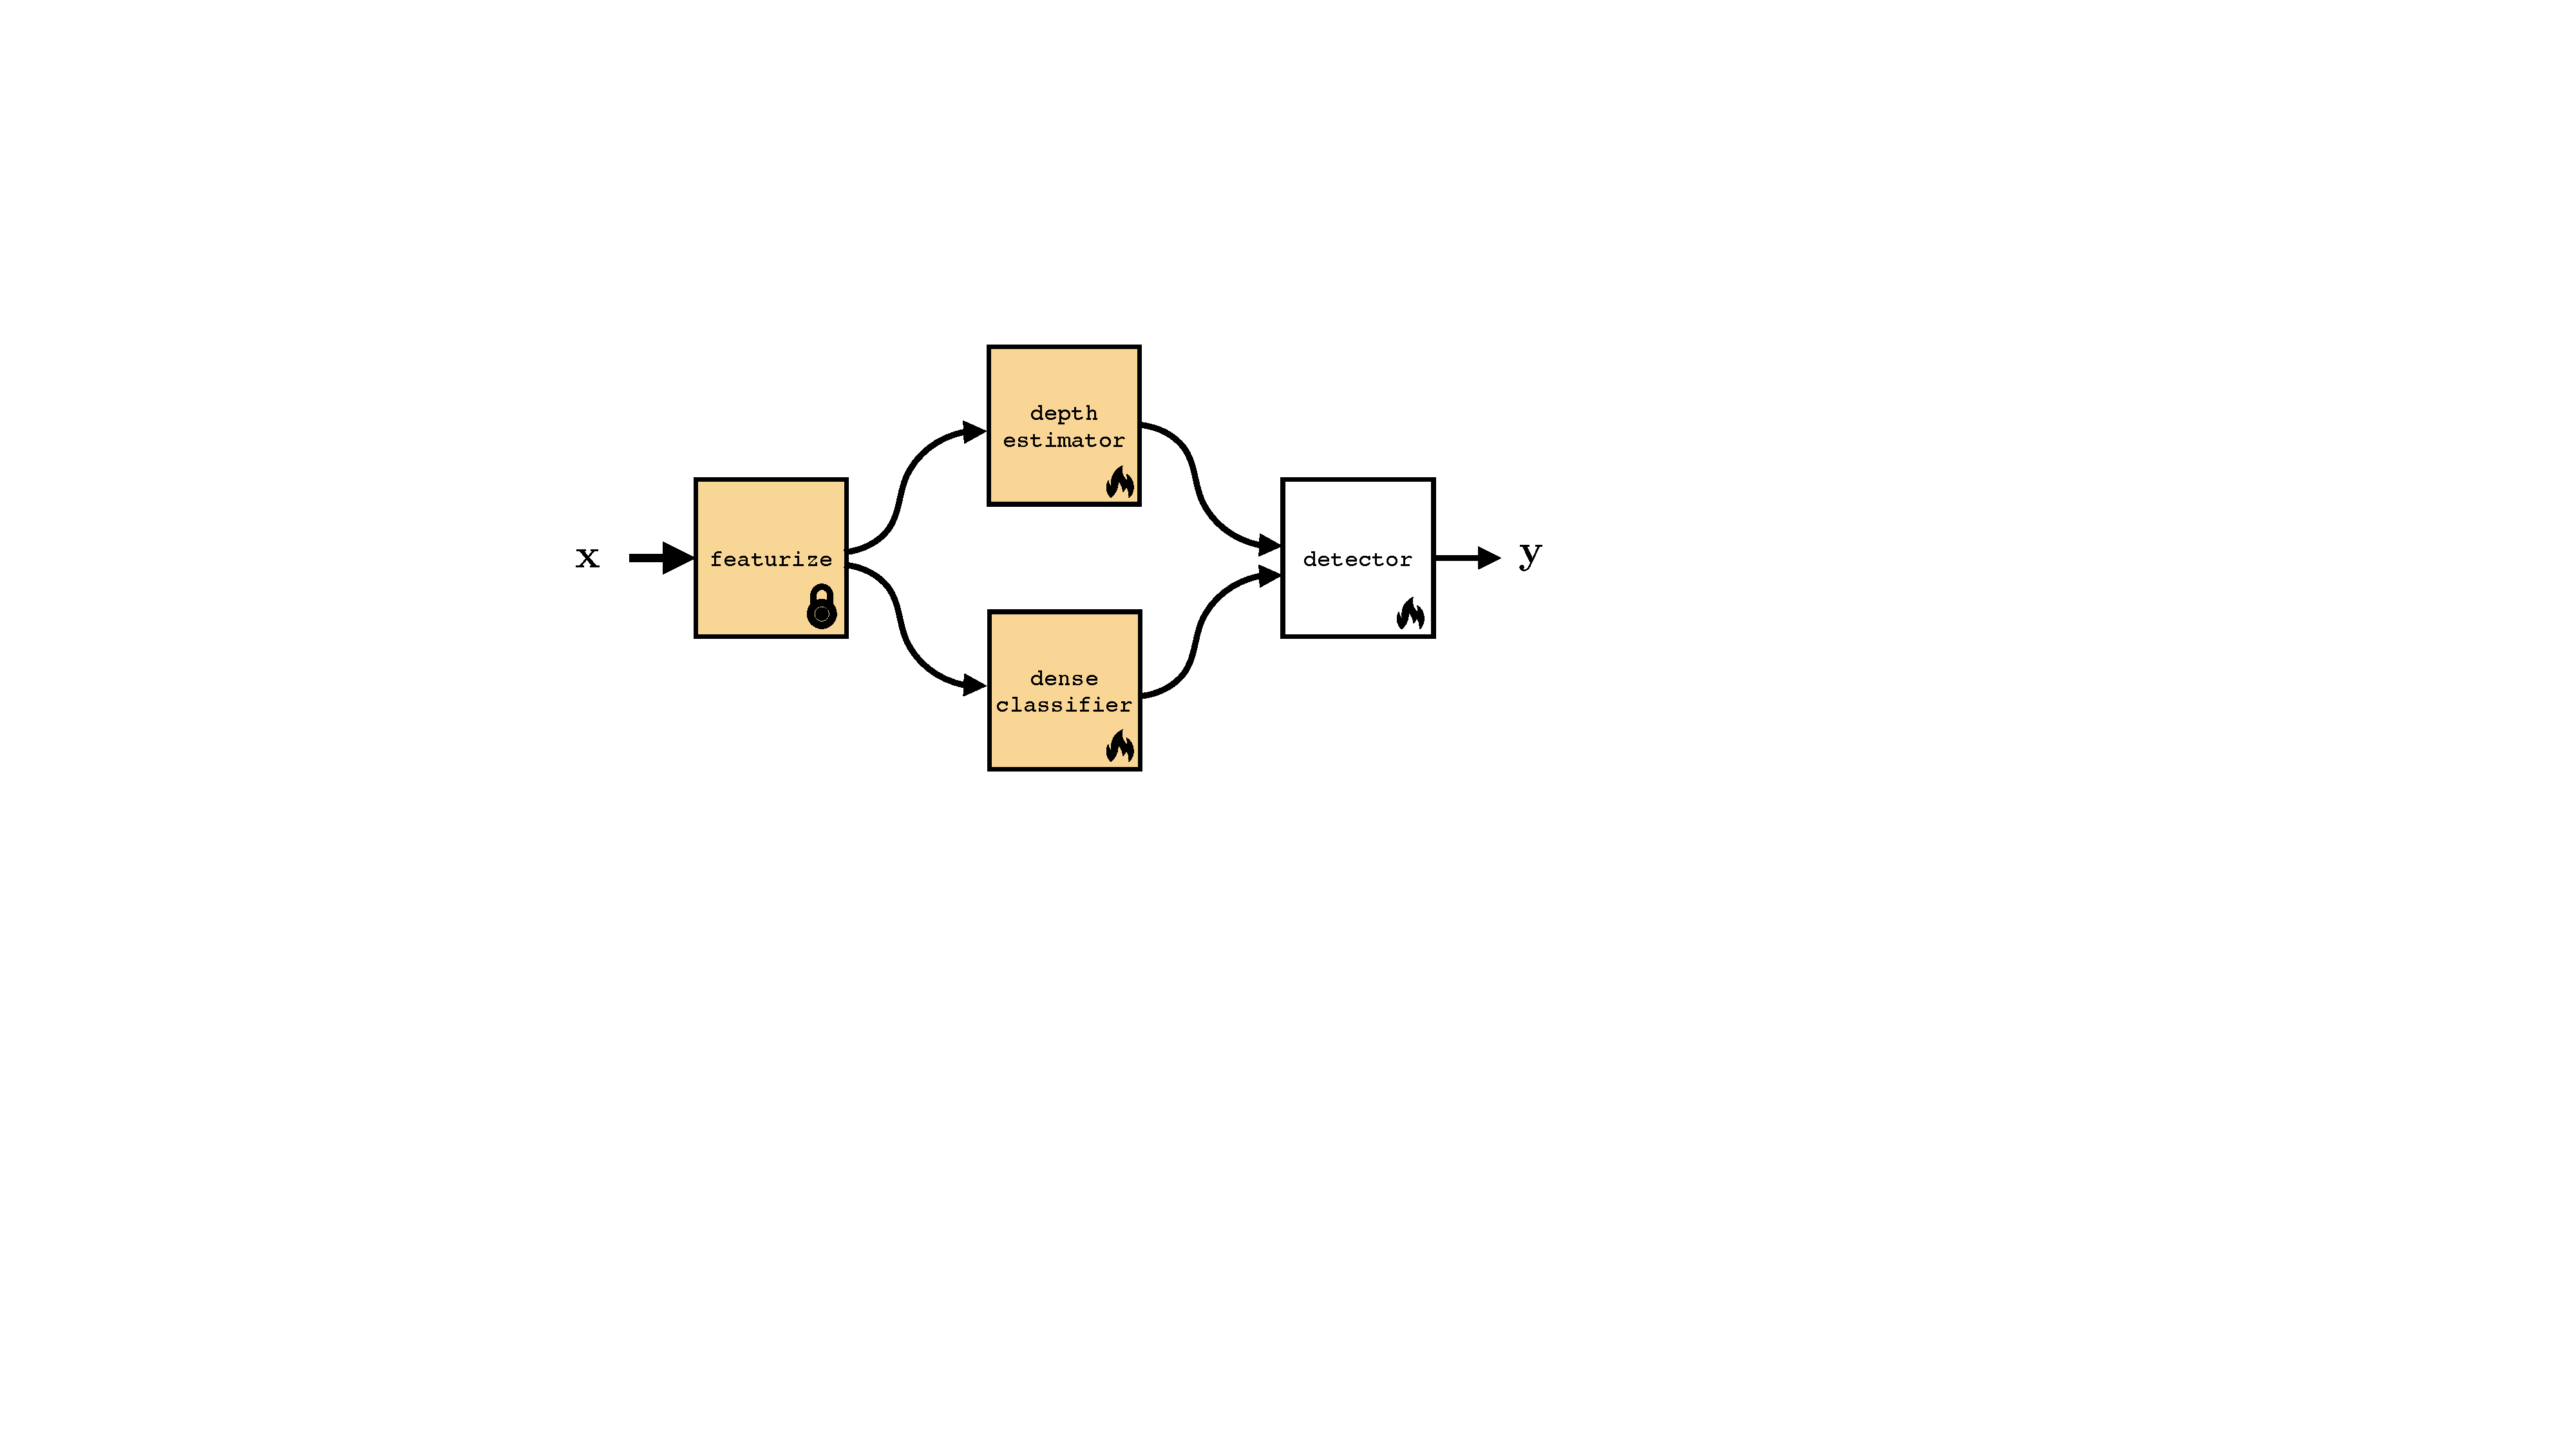
\includegraphics[width=0.7\linewidth]{./figures/transfer_learning/finetuning_certain_modules_example.pdf}
    }
    \caption{Finetuning certain subsets of a computation graph. Here we show some modules that have been pretrained (those with a shaded background) and one that is trained from scratch at finetuning time.}
    \label{fig:transfer_learning:finetuning_certain_modules_example}
\end{figure}

Within a single layer, it is also possible to update just a subspace of the full weight matrix. This can be an effective way to save memory (fewer weight gradients to track during backpropagation) or to regularize the amount of adaptation you are performing. One popular way to do so is to apply a low-rank update to the weight matrix~\cite{hu2021lora}.

\subsection{Heads and Probes}
As discussed previously, a model can be adapted by changing some or all of its parameters, or by adding entirely new modules to the computation graph. One important kind of new module is a \index{Read out module}\textbf{read out} module that takes some features from the computation graph as input and produces a new prediction as output. When these modules are linear, they are called \index{Linear probe}\textbf{linear probes}. These modules are relatively lightweight (few parameters) and can be optimized with tools from linear optimization (where there are often closed form solutions). Because of this, linear probes are very popular as a way of repurposing a neural net to perform a new task. These modules are also useful as a way of assessing what kind of knowledge each feature map in the original network represents, in the sense that if a feature map can linearly classify some attribute of the data, then that feature maps knows something about that attribute. In this usage, linear probes are probing the knowledge represented in some layer of a neural net.

%\subsection{Low-Rank Finetuning}


\section{Learning from a Teacher}
When we first encountered supervised learning in \chap{\ref{chapter:intro_to_learning}}, we described it as \textit{learning from examples}. You are given a dataset of example inputs and their corresponding outputs and the task is to infer the relationship that can explain these input-output pairs:
\begin{center}
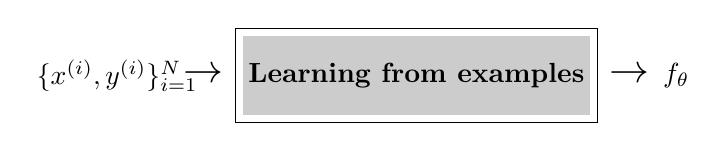
\begin{tikzpicture}
    \draw (0,1.2) rectangle (4.6,2.4); % outer box
    \fill[black!20] (0.1,1.3) rectangle (4.5,2.3); % gray box
    \node[] at (2.3,1.8) {{\bf Learning from examples}};
    %\node[] at (-1.5,2.4) {Data};
    \node[] at (-1.5,1.8) {$\{x^{(i)}, y^{(i)}\}_{i=1}^N$};
    \node[] at (-0.4,1.8) {{\Large  $ \rightarrow$}};
    \node[] at (5.6,1.8) {{$f_{\theta}$}};
    \node[] at (5.0,1.8) {{\Large  $ \rightarrow$}};
\end{tikzpicture}
\end{center}

This kind of learning is like having a very lazy teacher, who just gives you the answer key to the homework questions but does not provide any explanations and won't answer questions. Taking that analogy forward, could we learn instead from a more instructive teacher?

One way of formalizing this setting is to consider the teacher as a well-trained model $t: \mathcal{X} \rightarrow \mathcal{Y}$ that maps input queries to output answers. The student (the learner) observes both data $\{x^{(i)}\}^N_{i=1}$ and has access to the teacher model $t$. The student can learn to imitate the teacher's outputs or can learn to match \textit{how the teacher processes the queries}, matching intermediate activations of the teacher model.
\begin{center}
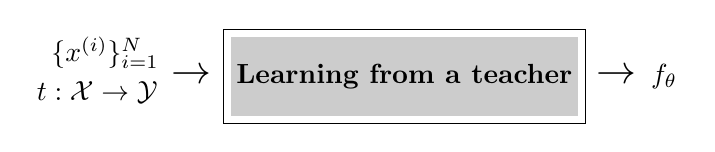
\begin{tikzpicture}
    \draw (0,1.2) rectangle (4.6,2.4); % outer box
    \fill[black!20] (0.1,1.3) rectangle (4.5,2.3); % gray box
    \node[] at (2.3,1.8) {{\bf Learning from a teacher}};
    %\node[] at (-1.5,2.4) {Data};
    \node[] at (-1.5,2.1) {$\{x^{(i)}\}_{i=1}^N$};
    \node[] at (-1.6,1.6) {$t: \mathcal{X} \rightarrow \mathcal{Y}$};
    \node[] at (-0.4,1.8) {{\Large  $ \rightarrow$}};
    \node[] at (5.6,1.8) {{$f_{\theta}$}};
    \node[] at (5.0,1.8) {{\Large  $ \rightarrow$}};
\end{tikzpicture}
\end{center}
\marginnote{Learning from examples can be considered a special case of learning from a teacher. It is the case where the teacher is the world and our only access to the teacher is observing outputs from it, that is, the examples $y$ that match each input $x$.}[-2cm]

\subsection{Knowledge distillation}
\index{Knowledge distillation}\textbf{Knowledge distillation} is a simple and popular algorithm for learning a classifier from a teacher. We assume that the teacher is a well-trained classifier that outputs a $K-1$-dimensional probability mass function (pmf), $t: \mathcal{X} \rightarrow \vartriangle^{K-1}$ (see \sect{\ref{sec:intro_to_learning:image_classification}}). The student, a model $f_{\theta}: \mathcal{X} \rightarrow \vartriangle^{K-1}$, simply tries to imitate the teacher's output pmf: for each input $x$ that the student sees, its goal is to output the same pmf vector as the teacher outputs for $x$. The full algorithm is given in the diagram below.

\begin{center}
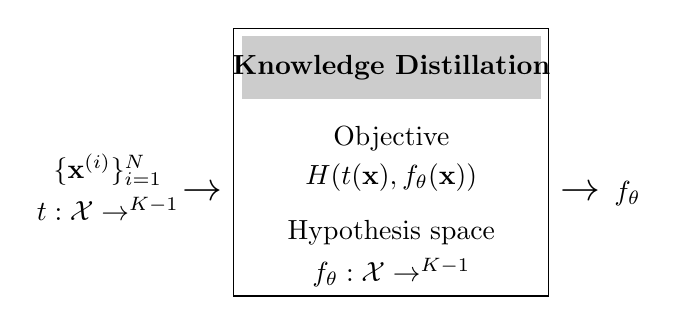
\begin{tikzpicture}
    \draw (0,-1.0) rectangle (4.0,2.4); % outer box
    \fill[black!20] (0.1,1.5) rectangle (3.9,2.3); % gray box
    \node[] at (2,1.9) {{\bf Knowledge Distillation}};
    \node[] at (2,1.0) {Objective}; \node[] at (2,0.5) {$H(t(\mathbf{x}), f_{\theta}(\mathbf{x}))$}; %\node[] at (2.5,0.0) {$\mathbf{y}_t  = \texttt{softmax}(t(\mathbf{x})), \hat{\mathbf{y}} = \texttt{softmax}(f_{\theta}(\mathbf{x}))$};
    \node[] at (2,-0.2) {Hypothesis space}; \node[] at (2,-0.7) {$f_{\theta}: \mathcal{X} \rightarrow \vartriangle^{K-1}$};
    %\node[] at (-1.6,0.9) {Inputs};
    \node[] at (-1.6,0.6) {$\{\mathbf{x}^{(i)}\}_{i=1}^N$};
    \node[] at (-1.6,0.1) {$t: \mathcal{X} \rightarrow \vartriangle^{K-1}$};
    \node[] at (-0.4,0.3) {{\Large  $ \rightarrow$}};
    \node[] at (5.0,0.3) {{$f_{\theta}$}};
    \node[] at (4.4,0.3) {{\Large  $ \rightarrow$}};
\label{fig:transfer_learning:knowledge_distillation_learning_problem}
\end{tikzpicture}
\end{center}
%\marginnote{\texttt{KD} for transferring knowledge from the logits of a $K$-way classifier, formulation from \cite{XX}.}[-3cm]
\marginnote{This section describes knowledge distillation as it was defined in \cite{hinton2015distilling}, which is the paper that introduced the term. Note that the term is now often used to refer to the whole family of algorithms that have extended this original method. See \cite{gou2021knowledge} for a survey.}[-2cm]



%\textbf{Knowledge distillation} transfers \textit{prediction targets} from one learning problem to another. This is useful whenever the second learner is somehow less privileged than the first.

%The idea is to look at how the teacher \textit{processes} the data and learn from that. We will describe the simplest and most popular version of this idea, from \cite{hinton2015distilling}, but note that there are many hundreds of published variations on this theme (see \cite{gou2021knowledge} for a survey). We will call \cite{hinton2015distilling}'s knowledge distillation algorithm \texttt{KD}.

%In \texttt{KD}, the student learns from the \textit{logits} output by the teacher (note that \texttt{KD} only applies to classification problems). The objective for the student is to minimize the difference between its logit vector and the teacher's logit vector, for the same input image.

\begin{figure}[h!]
    \centerline{
    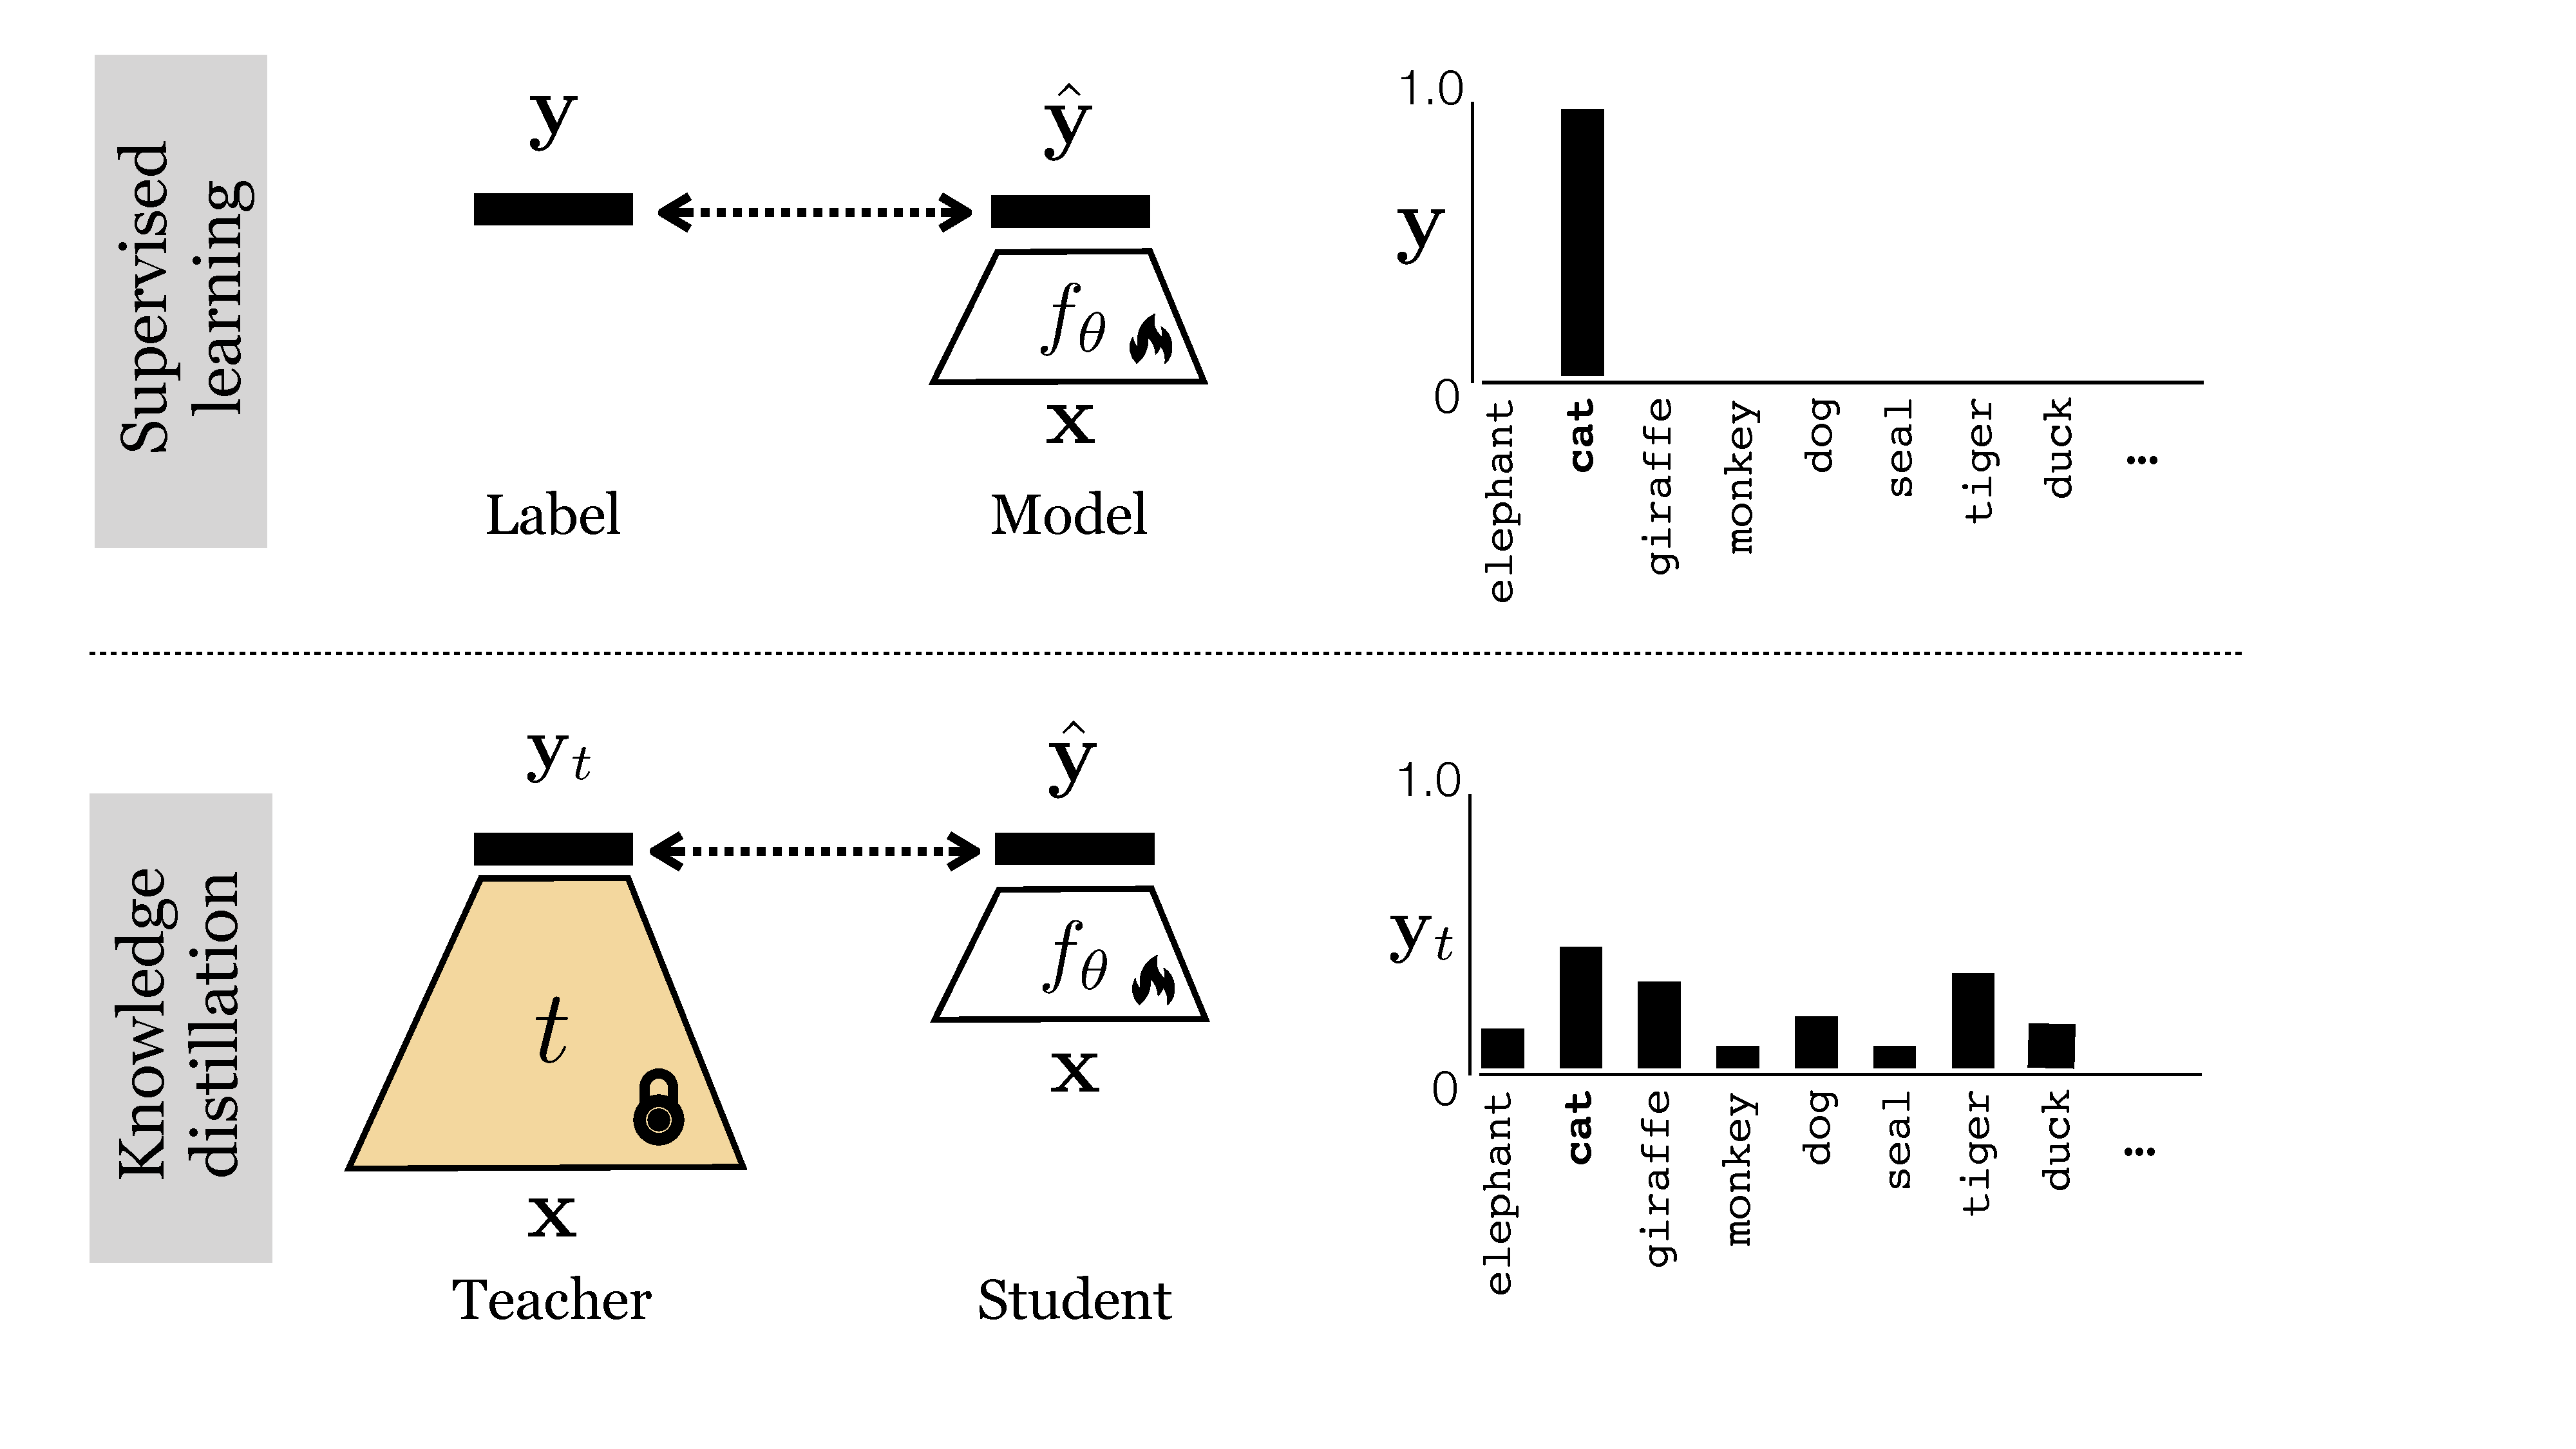
\includegraphics[width=1.0\linewidth]{./figures/transfer_learning/KD_diagram.pdf}
    }
    \caption{Comparing knowledge distillation to supervised learning from labels.}
    \label{fig:transfer_learning:KD_diagram}
\end{figure}

Notice that this learning problem is very similar to softmax regression on labeled data, and a diagram comparing the two is given in \fig{\ref{fig:transfer_learning:KD_diagram}}. The difference is that in knowledge distillation the targets are not one-hot (like in standard label prediction problems) but rather are more \textit{graded}.  %The difference is that 1) the supervision occurs on the \textit{logits} rather than on the normalized outputs, and 2) the targets are not one-hot (like in standard label prediction problems) but rather are more \textit{graded}. 
The teacher outputs a probability vector that reflect the teacher's belief as to the class of the input, rather than the ground truth class of the input. These beliefs may assign partial credit to classes that are similar to the ground truth, and this can actually make the teacher \textit{more} informative than learning from ground truth labels.

Think of it this way: the ground truth label for a domestic cat is ``domestic cat'' but the pmf vector output by a teacher, looking at a domestic cat, is more like ``this image looks 90 percent like a domestic cat, but also 10 percent like a tiger.'' That would be rather informative if the domestic cat in the image is a particularly large and fearsome looking one. The student not only gets to learn that this image is showing a domestic cat but also that this particular domestic cat is tiger-like. That tells the student something about both the class ``domestic cat'' and the class ``tiger.'' In this way the teacher can provide more information about the image than a one-hot label would, and in some cases this extra information can accelerate student learning~\cite{hinton2002training}.

%Here is a simple experiment where that happens.



%In most of this book, we have studied learning as the problem of extracting lessons from a training \textit{dataset} $\{x^{(i)}, y^{(i)}\}_{i=1}^N$, which we could call ``learning from data." But a dataset isn't the only kind of signal one can learn from. Another kind of learning involves having access to a \textit{teacher} that you can ask questions of, which we will call ``learning from a teacher." 

%Learning from data is the special case where the teacher wrote a textbook and then retired -- you can't ask them any new questions and have to rely on just reading through the questions they have already answered. For learning from data, implicitly, there is some function $t$ that produced the targets $y$, but we don't have access to that function (often that function is the world or physics).

%Knowledge distillation is a way to train one model to imitate the behavior of another. 

\section{Prompting}
\index{Prompting}

Prompting edits the \textit{input data} to solve a new problem. Prompting is very popular in natural language processing (NLP), where text-to-text systems can have natural language prompts prepended to the string that is input to the model. For example, a general-purpose language model can be prompted with [\texttt{Make sure to answer in French}, \texttt{X}], for some arbitrary input \texttt{X}. Then the output will be a French translation of whatever the model would have responded to when queried with \texttt{X}.

The same can be done for vision systems. First, prompting methods from NLP can be directly used for prompting the text inputs to vision-language models~\cite{radford2021learning} (\sect{\ref{sec:VLMs:CLIP}}). Second, prompting can also be applied to visual inputs. Just like we can prepend a textual input with text, we can prepend a visual input with visual data, yielding a method that may be called \textbf{visual prompting}~\cite{bahng2022exploring,bar2022visual,jia2022visual}. This can be done by concatenating pixels, tokens, or other visual formats to a vision model's inputs. This requires a model that takes variable-sized inputs; luckily this includes most neural net architectures, such as convolutional neural nets (CNNs), recurrent neural nets (RNNs), and transformers. Or, we can combine the visual prompt with the input query in other ways, such as by addition. 

Prompting is visualized in \fig{\ref{fig:transfer_learning:prompting}}, where $\oplus$ represents concatenation, addition, or potentially other ways of mixing prompts and input signals.
\begin{figure}[h!]
    \centerline{
    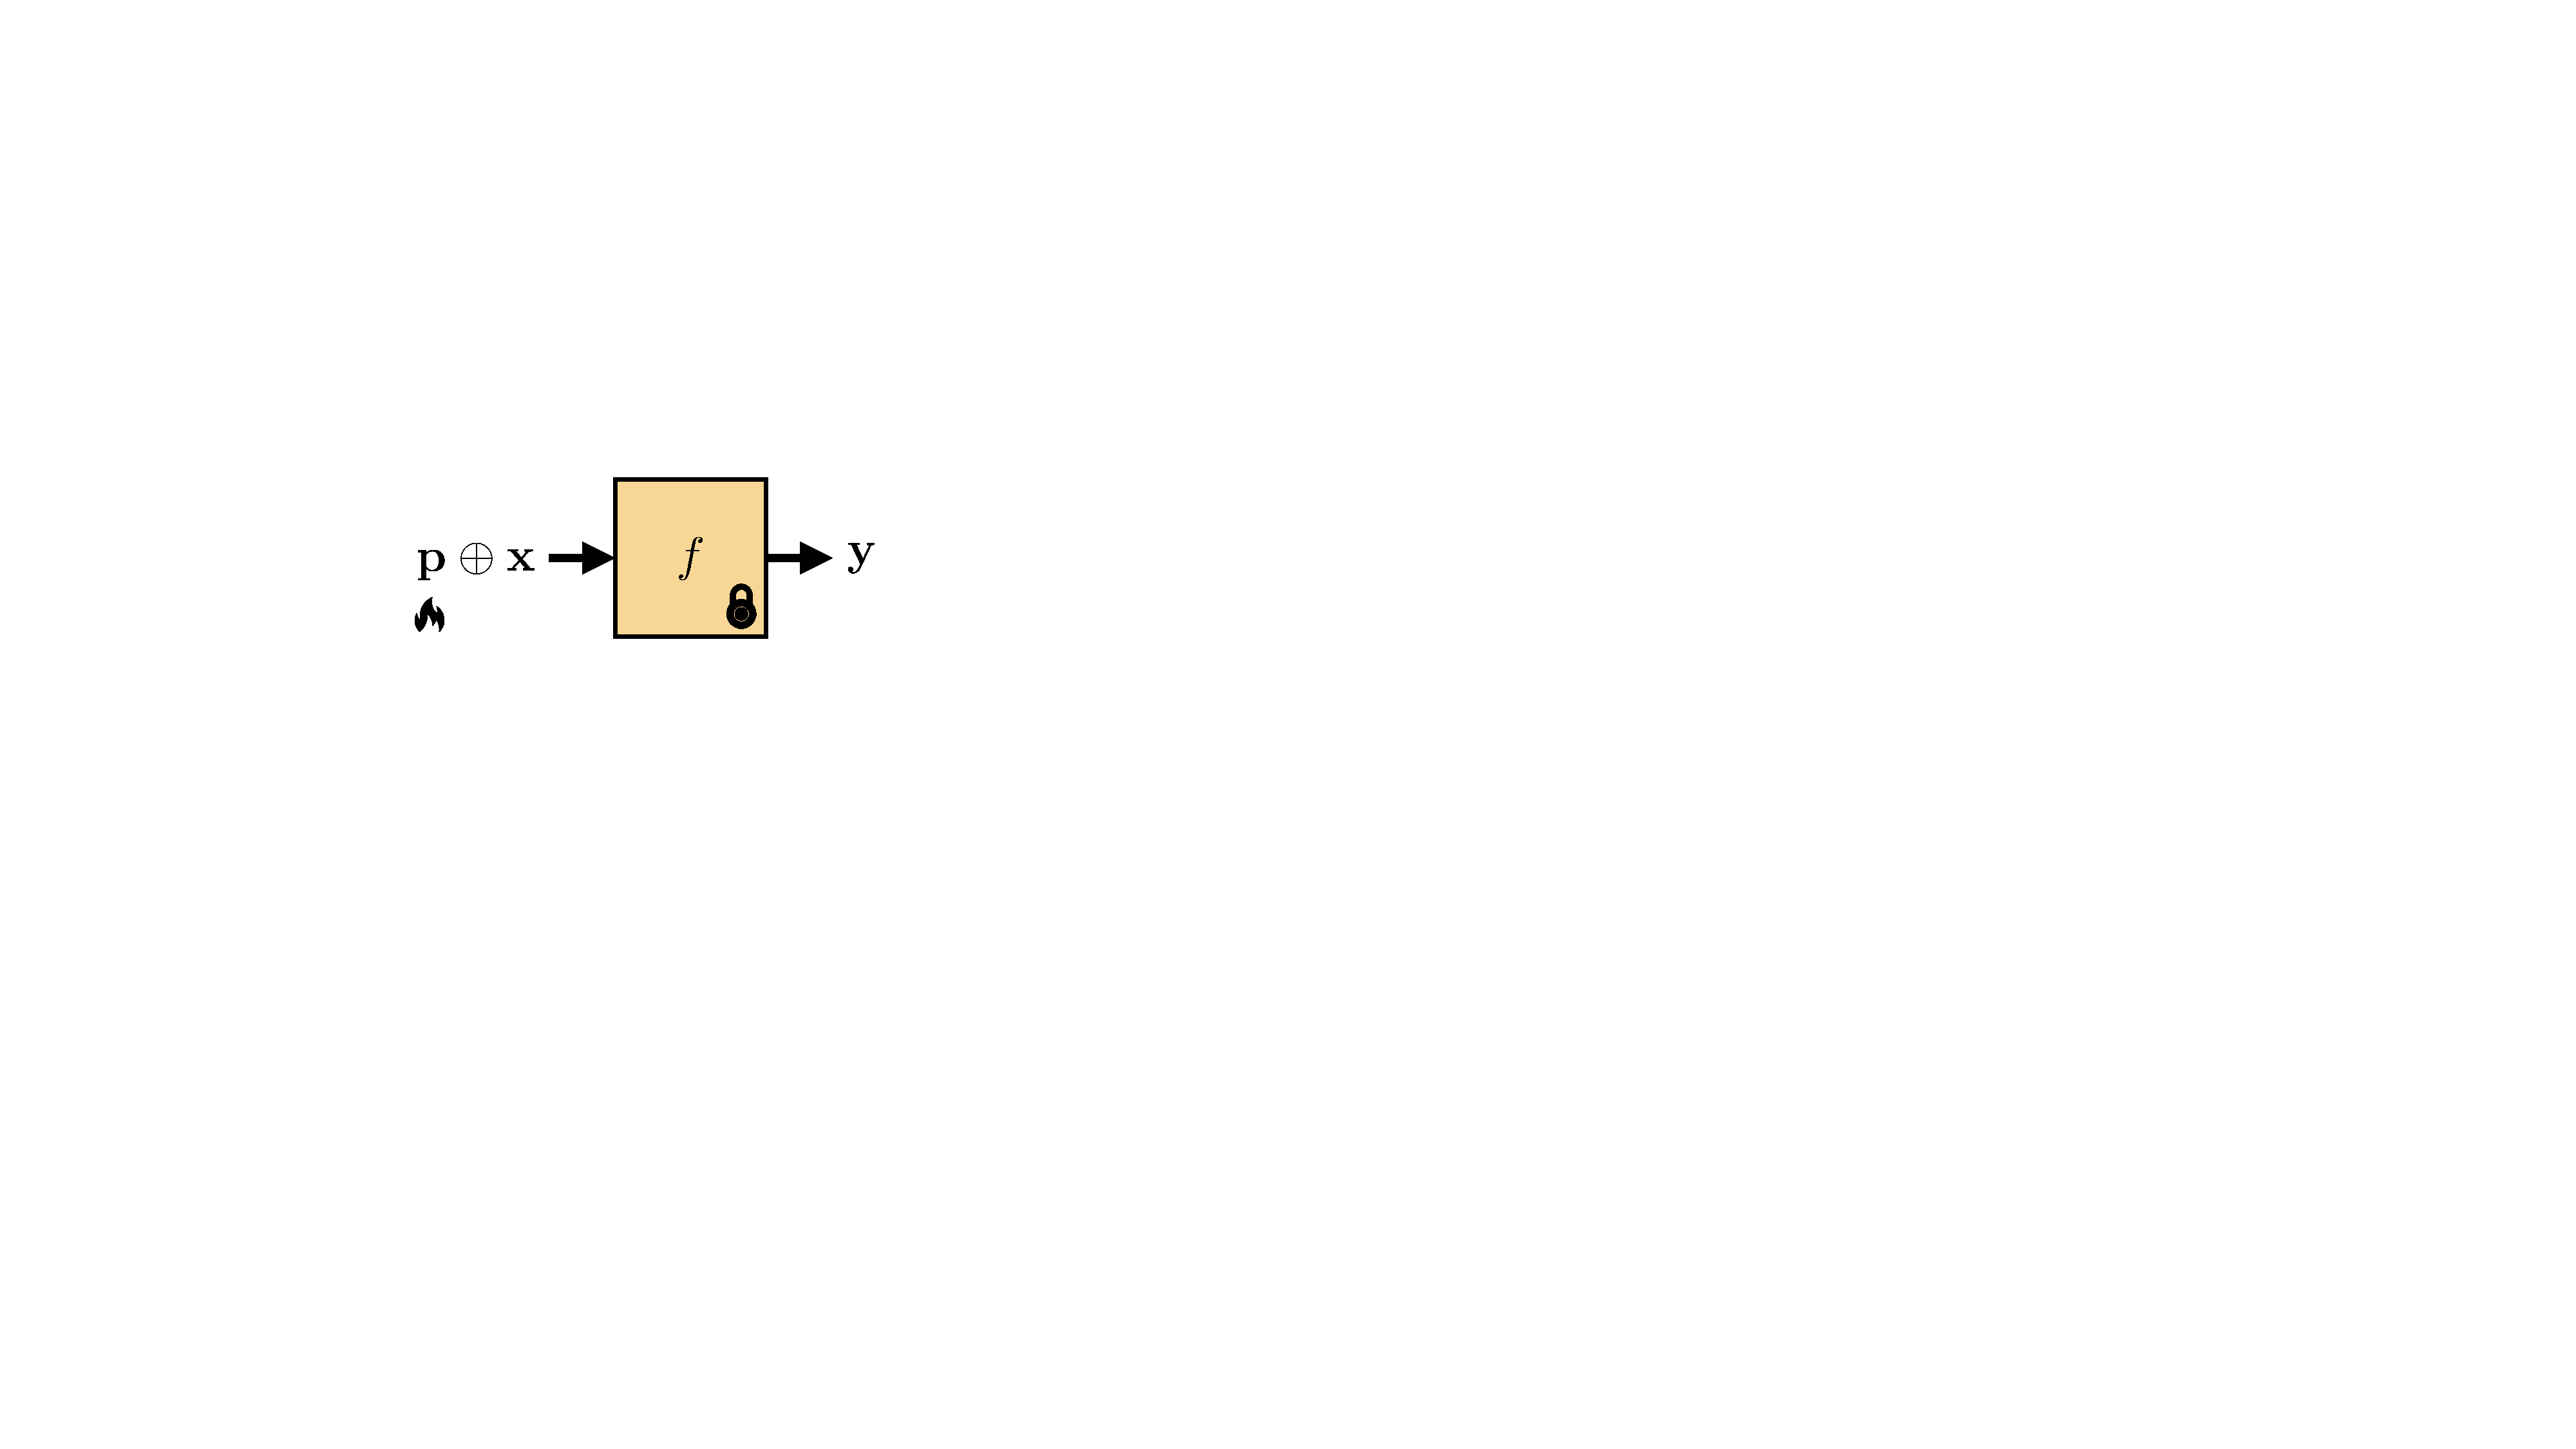
\includegraphics[width=0.35\linewidth]{./figures/transfer_learning/prompting.pdf}
    }
    \caption{Prompting: a prompt $\mathbf{p}$ is combined with the input $\mathbf{x}$ to change the output $\mathbf{y}$.}
    \label{fig:transfer_learning:prompting}
\end{figure}

Let's now look at several concrete ways of prompting a vision system. One simple way is to directly edit the input pixels, and this approach is shown in \fig{\ref{fig:transfer_learning:pixel_prompt}}:
\begin{figure}[h!]
    \centerline{
    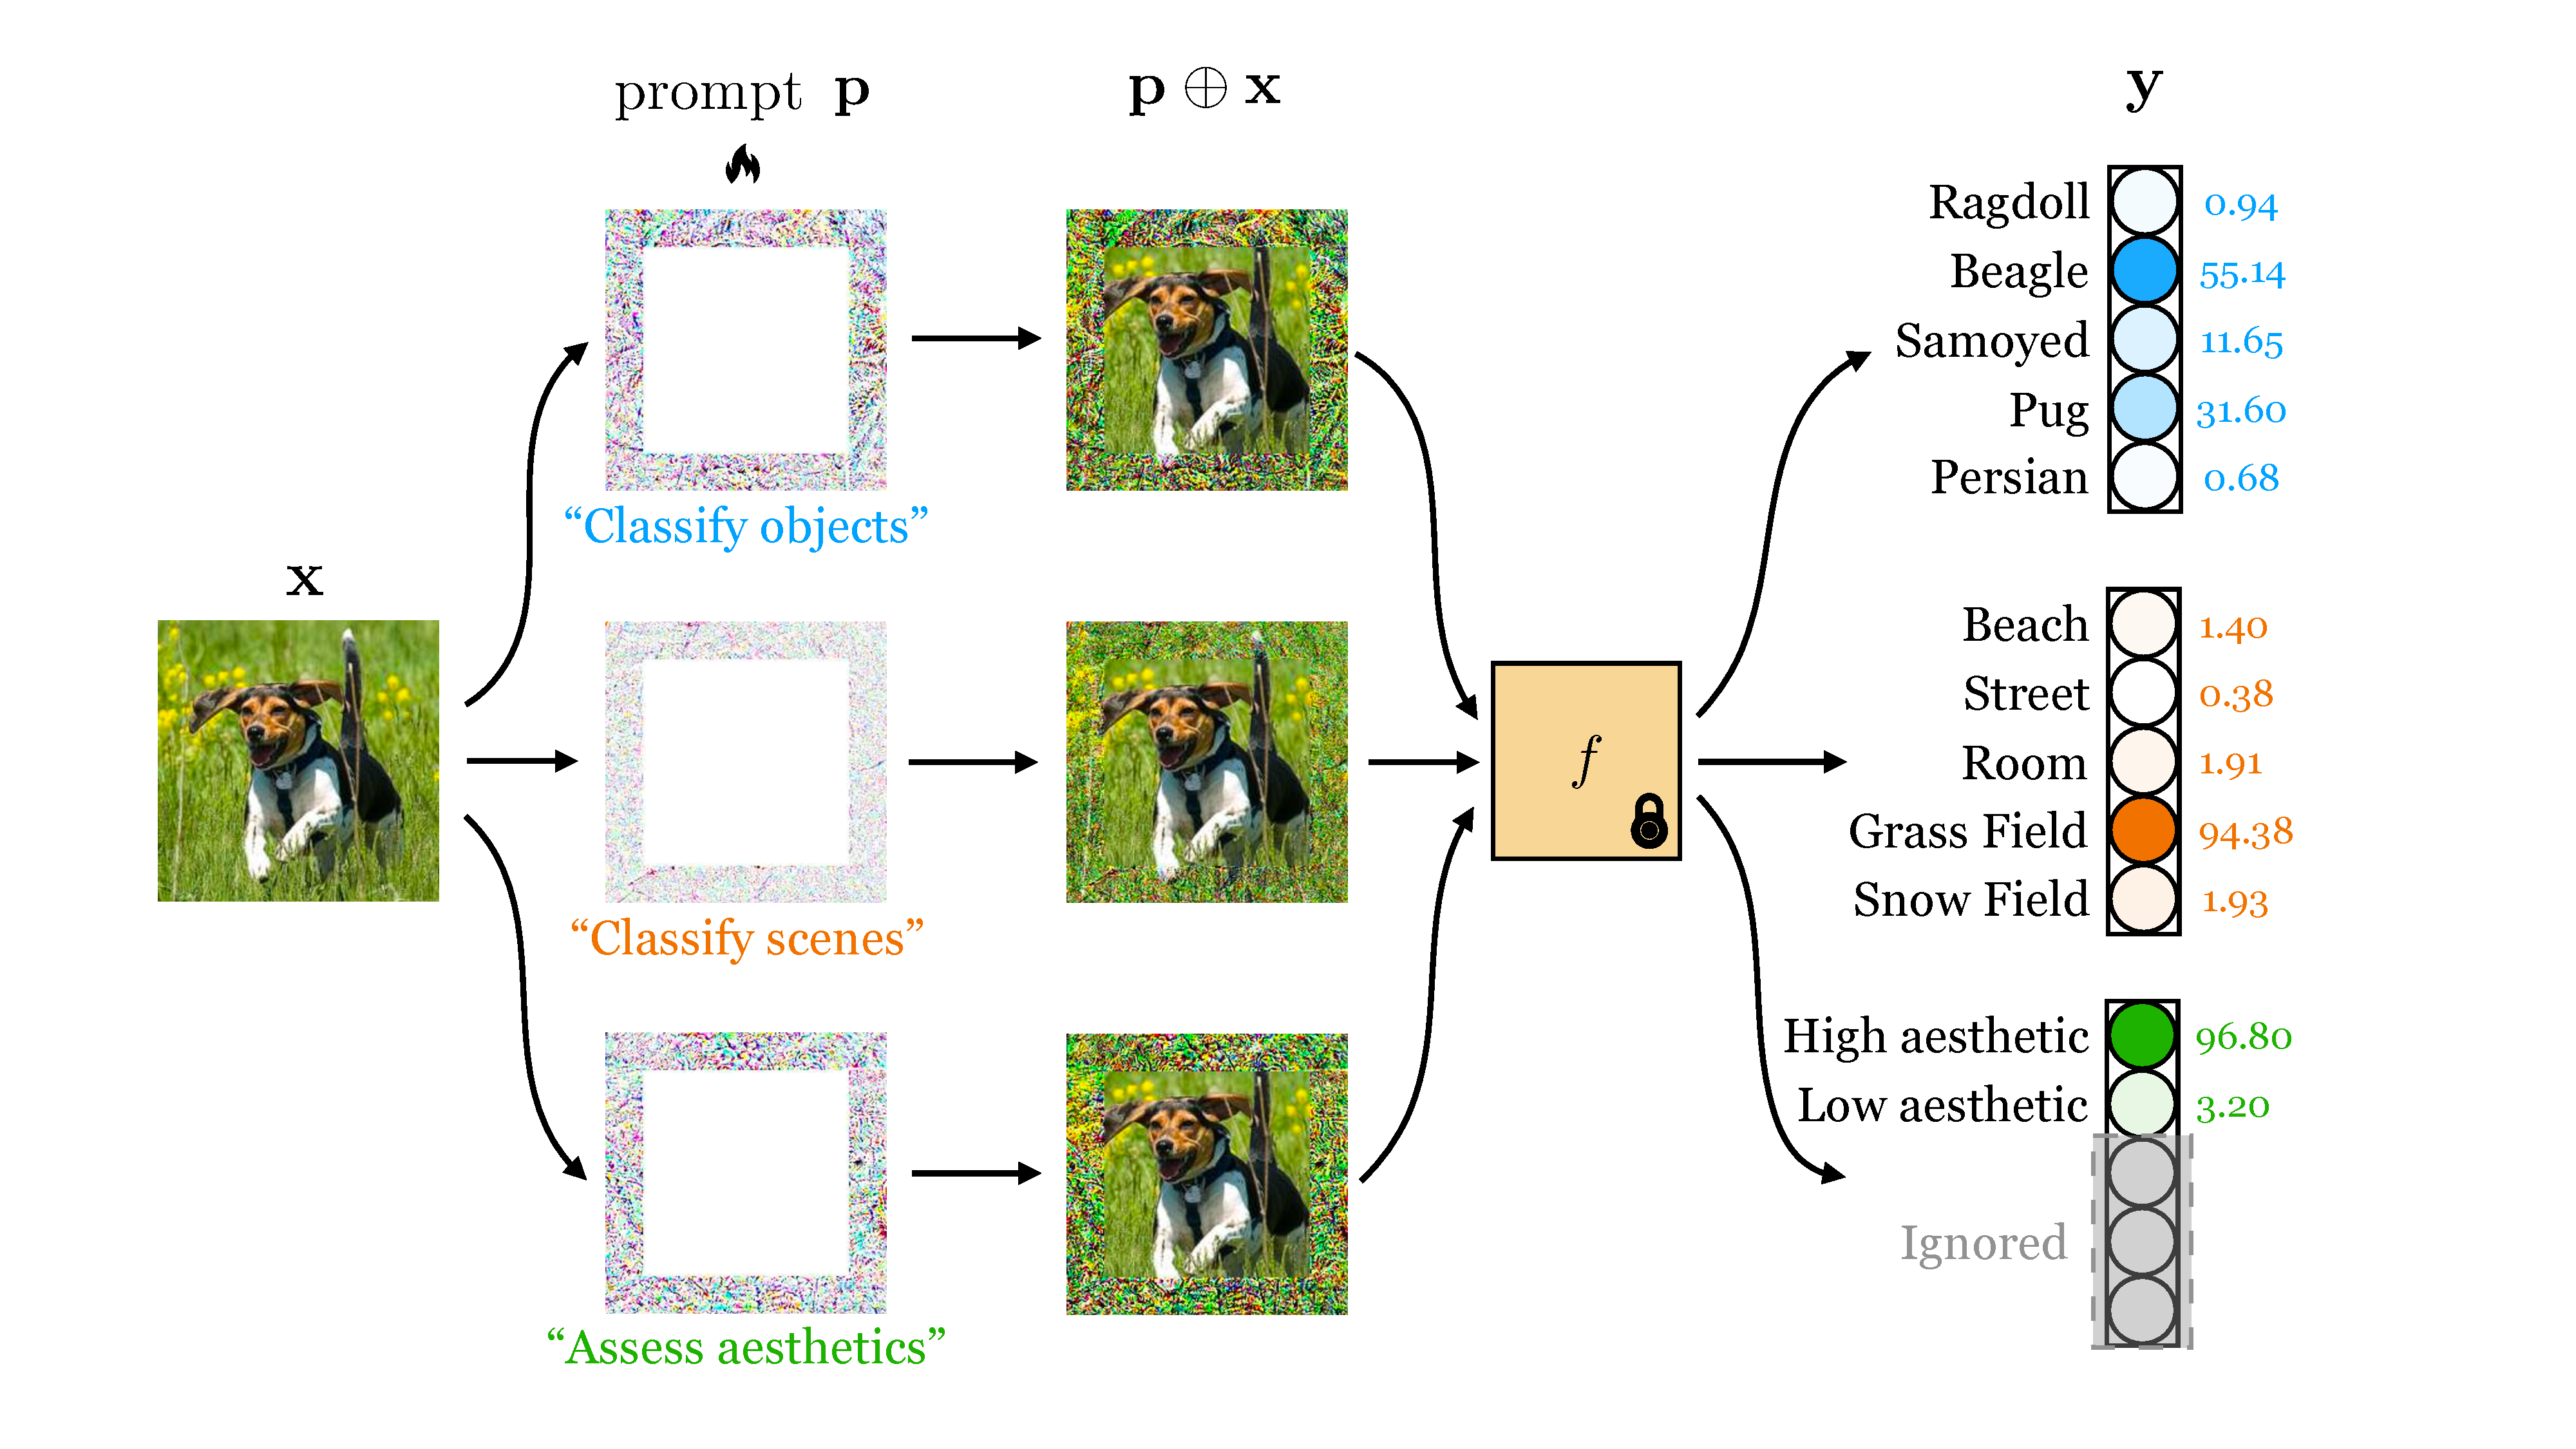
\includegraphics[width=1.0\linewidth]{./figures/transfer_learning/vp_hyojin.pdf}
    }
    \caption{A prompt can be made out of pixels: a prompt image (which looks like a border of noise here) is added to the input image in order to change the model's behavior. Three different prompts are shown, one that adapts the model to perform scene classification, a second for aesthetics classification, and a third for object classification. Modified from \cite{bahng2022exploring}.}
    \label{fig:transfer_learning:pixel_prompt}
\end{figure}

Here, the prompt is an image $\mathbf{p}$ that is added to the input image $\mathbf{x}$. The prompt looks like noise, but it is actually an optimized signal that changes the model's behavior. The top prompt was optimized to make the model predict the dog's species and the bottom prompt was optimized to make the model predict the dog's expression. Mathematically, this kind of prompting is very similar to the adversarial noise we covered in \sect{\ref{sec:bias_and_shift:adversarial_attacks}}. \marginnote{Because of its similarity to adversarial examples, early papers on prompting sometimes referred to it as \textbf{adversarial reprogramming}~\cite{elsayed2018adversarial}.}[-1.8cm]
However, here we are not adding noise that \textit{hurts} performance but instead adding noise that \textit{improves} performance on a new task of interest. Given a set of $M$ training examples that we would like to adapt to, $\{\mathbf{x}^{(i)}, \mathbf{y}^{(i)}\}_{i=1}^M$, we learn a prompt via the following optimization problem:
\begin{align}
    \argmin_{\mathbf{p}} \sum_{i=1}^M \mathcal{L}(f(\mathbf{x}^{(i)} + \mathbf{p}), \mathbf{y}^{(i)})
\end{align}
where $\mathcal{L}$ is the loss function for our problem.\footnote{Here we require that the output space $\mathcal{Y}$ is the same between the pretrained model and the prompted model. If we want to adapt to perform a task with a different output dimensionality then we can add a learned projection layer $f^{\prime}$ after the pretrained $f$, just like we did in \fig{\ref{fig:transfer_learning:finetuning_stages}}.}

Rather than adding a prompt in pixel space, it is also possible to add a prompt to an intermediate feature space. Let's look next at one way to do this. Jia, Tang, \textit{et al.}~\cite{jia2022visual} proposed to use a \textit{token} as the prompt for a vision transformer architecture~\cite{dosovitskiy2020vit} (see \chap{\ref{chapter:transformers}} for details on transformers). This new token is concatenated to the input of the transformer, which is a set of tokens representing image patches (\fig{\ref{fig:transformers:prompting_a_transformer}}):
\begin{figure}[h]
\centerline{
\begin{tikzpicture}
%
\def\Nnodes{3}
\def\Nlayers{3}
\def\layerheight{1.2}
\def\neuronrad{0.3}
\def\neuronstep{0.7}
% prompt
\draw (-\neuronrad/4,-\neuronrad) rectangle ++(\neuronrad/2,\neuronrad*2);
\node at (0,-\neuronrad*1.75) {
\includegraphics[width=0.03\linewidth]{./figures/transfer_learning/fire.png}};
\draw (0,-\neuronrad*3) node {prompt};
\foreach \xj in {1,...,\Nnodes} {
    \draw [thick] [nn_edge] (0,\neuronrad) -- (\neuronstep*\xj,\layerheight-\neuronrad);
}
% inputs
\foreach \x in {1,...,\Nnodes} {
    \foreach \y in {1,...,\Nlayers} {
        \draw (\neuronstep*\x-\neuronrad/4,\layerheight*\y-\layerheight-\neuronrad) rectangle ++(\neuronrad/2,\neuronrad*2);
    }
}
% mixing layer 1
\foreach \xi in {1,...,\Nnodes} {
    \foreach \xj in {1,...,\Nnodes} {
        \draw [thick] [nn_edge] (\neuronstep*\xi,\neuronrad) -- (\neuronstep*\xj,\layerheight-\neuronrad);
    }
}
% pointwise nonlinearity
\foreach \x in {1,...,\Nnodes} {
    \draw [thick] [nn_edge] (\neuronstep*\x,\layerheight+\neuronrad) -- (\neuronstep*\x,\layerheight*2-\neuronrad);
}
\draw [thick] [nn_edge] (2.5,0) arc
    [
        start angle=-70,
        end angle=90,
        x radius=0.4cm,
        y radius =0.3cm
    ] ;
\draw (2.4, 0) node {$\Big\}$};
\draw (3.3,0.25*\layerheight) node {$\texttt{attn}$};
\end{tikzpicture}
}
\caption{Prompting a transformer with a learnable input token. The prompt token is mixed into the network via attention; therefore \textit{no} parameters of the original network have to be updated (see \chap{\ref{chapter:transformers}}).}
\label{fig:transformers:prompting_a_transformer}
\end{figure}

The token is a $d$-dimensional code vector and this vector is optimized to change the behavior of the transformer to achieve a desired result, such as increased performance on a new dataset or task. The attention mechanism works as usual except now all the input tokens also attend to the prompt. The prompt thereby modulates the transformation applied to the input tokens on the first layer, and this is how it affects the transformer's behavior.

It is also possible to train a model to be \textit{promptable}, so that at test time it adapts better to user prompts. An advantage of this approach is that we can train a model to understand human-interpretable prompts. For example, we could train the model so that its behavior can be adapted based on text instructions or based on user-drawn strokes (a representative example of both of these use cases can be found in \cite{kirillov2023segment}). In fact, we have already seen many such systems in this book: any system that interactively adapts to user inputs can be considered a promptable system. In particular, many promptable systems use the tools of conditional generative modeling (\chap{\ref{chapter:conditional_generative_models}}) to train systems can are conditioned on user text instructions (e.g., \cite{dalle1}, \cite{rombach2022high}, which we cover in \chap{\ref{chapter:VLMs}}).

%Then the prompt can be user inputs such as strokes and the training demonstrates how to interpret these user inputs. This is another name for a conditional model.
% SAM fig

% Our we can have a general purpose model that knows how to complete sequences like humans do in figures, and then you can prompt that...
% Efros fig


\section{Domain Adaptation}
\index{Domain adaptation}

Often, the data we train on comes from a different distribution, or domain, than the data we will encounter at test time. For example, maybe we have trained a recognition system on internet photos and now we want to deploy the system on a self-driving car. The imagery the car sees looks very different than everyday photos you might find on the internet. \textbf{Domain adaptation} refers to methods for adapting the training domain to be more like the test domain, or vice versa.
%\textbf{Domain adaptation} refers to the setting where the input data distribution changes, i.e. $\mathcal{X} \neq \mathcal{X}^{\prime}$. 

%Finetuning is one example of domain adaptation, where the model $f$ is adapted by making use of labeled data in the test domain. But $f$ is not the only thing we can adapt. 
The first option is to adapt the test data, $\{\mathbf{x}_{\texttt{test}}^{(i)},\mathbf{y}_{\texttt{test}}^{(i)}\}_{i=1}^N$ to look more like the training data. Then $f$ should work well on both the training data and the test data. Or we can go the other way around, adapting the training data to look like the test data, \textit{before} training $f$ on the adapted training data. In either case, the trick is to make the distribution of test and train data identical, so that a method that works on one will work just as well on the other.

Commonly, we only have access to labels at training time, but may have plentiful unlabeled inputs $\{\mathbf{x}^{\prime}_i\}_{i=1}^N$ at testing time. This setting is sometimes referred to as \textbf{unsupervised domain adaptation}. Here we cannot make use of test labels but we can still align the test inputs to look like the training inputs (or vice versa). One way to do so is to use a generative adversarial network (GAN; \chap{\ref{chapter:generative_models}}) that translates the data in one domain to look identically distributed as the data in the other domain, as has been explored in e.g., \cite{tzeng2017adversarial,CycleGAN2017,hoffman2018cycada}. A simple version of this algorithm is given in \algref{\ref{alg:transfer_learning:domain_adaptation_by_translation}}.
% There are two general ways we can achieve alignment between two domains:
% \begin{itemize}
%     \item Map $\mathcal{X}_{\texttt{test}}$ to $\mathcal{X}_{\texttt{train}}$ (or vice versa)
%     \item Map $\mathcal{X}_{\texttt{train}}$ to $\mathcal{Z}$ and $\mathcal{X}_{\texttt{test}}$ also to $\mathcal{Z}$
% \end{itemize}
% The first option is a kind of \textbf{translation} from $\mathcal{X}_{\texttt{test}}$ to $\mathcal{X}_{\texttt{train}}$ whereas the second option is a mapping to a domain-invariant shared space.

%These options are schematized below:

\marginnote{You may notice that domain adaptation is very similar to prompting. Both edit the model's inputs to make the model perform better. However, while prompting's objective is to improve or steer model performance, domain adaptation's objective is to make the inputs look more familiar. This means domain adaptation is applicable even when we don't have access to the model or even know what the task will be.}[-6cm]

\begin{algorithm}[h]
\SetAlgoVlined
\DontPrintSemicolon
%\marginnote{{\bf Algorithm \ref{alg:transfer_learning:domain_adaptation_by_translation}}: Here we use a GAN to translate from one domain to the other. This algorithm could be improved by adding cycle-consistency constraints (see CycleGAN from \chap{\ref{chapter:conditional_generative_models}}~\cite{CycleGAN2017}) as was done in \cite{hoffman2018cycada}.}
\caption{{\bf Algorithm \ref{alg:transfer_learning:domain_adaptation_by_translation}}: Unpaired domain adaptation via adversarial translation. Here we use a GAN to translate from one domain to the other. This algorithm could be improved by adding cycle-consistency constraints (see CycleGAN from \chap{\ref{chapter:conditional_generative_models}},~\cite{CycleGAN2017}) as was done in \cite{hoffman2018cycada}.}
\fakealgorithmcaption{}
\label{alg:transfer_learning:domain_adaptation_by_translation}
{\bf Input:} training data $\{x_{\texttt{train}}^{(i)},y_{\texttt{train}}^{(i)}\}_{i=1}^N$, test data, $\{x_{\texttt{test}}^{\prime^{(i)}}\}_{i=1}^M$\;
{\bf Output:} trained model $F$\;
{\bf Train predictor on \texttt{train}:}
    $f = \argmin_{f} \mathbb{E}_{x_{\texttt{train}},y_{\texttt{train}}}[\mathcal{L}(f(x_{\texttt{train}}),y_{\texttt{train}})]$\;
{\bf Train translator $\mathcal{X}_{\texttt{test}}$ to $\mathcal{X}_{\texttt{train}}$:}
    $G = \argmin_g \max_d \mathbb{E}_{x_{\texttt{train}}}[\log d(x_{\texttt{train}}))] + \mathbb{E}_{x_{\texttt{test}}}[\log(1-d(g(x_{\texttt{test}}))]$\;
return $F = f \circ g$
\end{algorithm}


% \begin{algorithm}[h]
% \label{domain_adaptation_by_common_embedding}
% \SetAlgoVlined
% \DontPrintSemicolon
% \caption{Unpaired domain adaptation via common embedding}
% {\bf Input:} training data $\{x_{\texttt{train}}^{(i)},y_{\texttt{train}}^{(i)}\}_{i=1}^N$, test data, $\{x_{\texttt{test}}^{\prime^{(i)}}\}_{i=1}^M$\;
% {\bf Output:} trained model $F$\;
% {\bf Train common embedding:} \For{\upshape $k = 1, \dots, K_2$} {
%     $E = \argmin_E \max_D \mathbb{E}_{x_{\texttt{train}}}[\log D(E(x_{\texttt{train}})))] + \mathbb{E}_{x_{\texttt{test}}}[{1-D(E(x_{\texttt{test}}}))]$\;
% }
% {\bf Train predictor on embeddings of \texttt{train}:} \For{\upshape $k = 1, \dots, K_1$} {
%     $f = \argmin_{f} \mathbb{E}_{x_{\texttt{train}},y_{\texttt{train}}}[\mathcal{L}(f(E(x_{\texttt{train}})),y_{\texttt{train}})]$\;
% }
% return $F = f \circ E$
% \end{algorithm}



%How we achieve these mappings depends on the kind of data available to us. The data in the two domains may be paired or unpaired. In the paired setting we can do image-to-image translation using a paired loss. In the unpaired setting we need to do unpaired translation.



\section{Generative Data}
\index{Generative data}

Generative models (\chap{\ref{chapter:generative_models}}) produce synthetic data that looks like real data. Could this ability be useful for transfer learning? At first glance it may seem like the answer is no: Why use fake data if you have access to the real thing?

However, \textbf{generative data} (i.e., synthetic data sampled from a generative model) is not just a cheap copy of real data. It can be \textit{more} data, and it can be \textit{better} data. It can be \textit{more} data because we can draw an unbounded number of samples from a generative model. These samples are not just copies of the training datapoints but can interpolate and remix the training data in novel ways (\chap{\ref{chapter:generative_models}}). Generative models can also produce \textit{better} data because the data comes coupled with a procedure that generated it, and this procedure has structure that can be exploited to understand and manipulate the data distribution.

One such structure is latent variables (\chap{\ref{chapter:generative_modeling_and_representation_learning}}). Suppose you have generated a training set of outdoor images with a latent variable generative model. You want to train an object classifier on this data. You notice that the images never show a cow by a beach, but you happen to live in northern California where the cows love to hang out on the coastal bluffs. How can you adapt your training data to be useful for detecting these particular cows? Easy: just edit the latent variables of your model to make it produce images of cows on beaches. If the model is pretrained to produce all kinds of images, it may have the ability to generate cows on beaches with just a little tweaking.

It is currently a popular area of research to use large, pretrained generative models as data sources for many applications like this~\cite{jahanian2021generative,he2022synthetic,brooks2022instructpix2pix}. In this usage, you are transferring knowledge about \textit{data}, to accelerate learning to solve a new problem. The function being learned can be trained from scratch, but it is leveraging the generative model's knowledge about what images look like and how the world works.

%Generative data transfers knowledge about the input data to accelerate future problem solving on this same kind of data.


%\section{Meta-learning}

\section{Other Kinds of Knowledge that Can Be Transferred}

This chapter has covered a few different kinds of knowledge that can be pretrained and transferred. We have not aimed to be exhaustive. As an exercise, you can try the following: (1) download the code for your favorite learning algorithm, (2) pick a random line, (3) and figure out how you can pretrain whatever is being computed on that line. Maybe you picked the line that defines the loss function; that can be pretrained! The term for this is a \textbf{learned loss} (e.g., \cite{houthooft2018evolved}). Or maybe you picked the line \texttt{optim.SGD...} that defines the optimizer: the optimizer can also be pretrained. This is called a \textbf{learned optimizer} (e.g., \cite{andrychowicz2016learning}). It's currently less common to \textit{adapt} modules like these (they are usually just pretrained and then held fixed), but in principle there is no reason why you can't. Maybe you, reader, can figure out a good way to do so.


\section{A Combinatorial Catalog of Transfer Learning Methods}\label{sec:transfer_learning:combinatorial_catalog}

Many of the methods we introduced previously follow a similar format:
\begin{itemize}
    \item Pretrain one component of the system.
    \item Adapt that component and/or other components.
\end{itemize}

In \tab{\ref{tab:generative_models:types_of_gen_model}}, we present the relationship these methods by framing them all as empirical risk minimization with different components optimized during pretraining and/or during adaptation.

%Both these stages involve numerous choices and each choice results in a different transfer learning algorithm. The key questions for the pretraining stage are: 1) what kind prior knowledge should we acquire and 2) how should we acquire it? Let's start by illustrating with an example.

\begin{table}[h]
    \caption{Different kinds of transfer learning presented as empirical risk minimization (ERM).\textit{ Notes}: The $\oplus$ symbol indicates concatenation or addition (or other kinds of signal combination). Domain adaptation does not map neatly to ERM so we omit it here.}
    %\marginnote{{\bf Table \ref{tab:generative_models:types_of_gen_model}}: Different kinds of transfer learning presented as empirical risk minimization (ERM).\textit{ Notes}: The $\oplus$ symbol indicates concatenation or addition (or other kinds of signal combination). Domain adaptation does not map neatly to ERM so we omit it here.}
    %\faketablecaption{}
    \label{tab:generative_models:types_of_gen_model}
    \centering
    \begin{tabular}{l|l|l}
        Method & Learning & Inference\\
         & \textcolor{pretrained_color}{pretrained} / \textcolor{adapted_color}{adapted} / \textcolor{both_color}{both}& \\
        \hline
        Generative data & $\argmin_{\textcolor{adapted_color}{\theta}} \mathbb{E}_{\textcolor{pretrained_color}{x},\textcolor{pretrained_color}{y}}[\mathcal{L}(f_{\textcolor{adapted_color}{\theta}}(\textcolor{pretrained_color}{x}), \textcolor{pretrained_color}{y})]$ & $f_{\textcolor{adapted_color}{\theta}}(x)$\\
        Distillation & $\argmin_{\textcolor{adapted_color}{\theta}} \mathbb{E}_{x}[\mathcal{L}(f_{\textcolor{adapted_color}{\theta}}(x), \textcolor{pretrained_color}{t}(x))]$ & $f_{\textcolor{adapted_color}{\theta}}(x)$\\
        Prompting & $\argmin_{\textcolor{adapted_color}{\epsilon}} \mathbb{E}_{x,y}[\mathcal{L}(f_{\textcolor{pretrained_color}{\theta}}(x \oplus \textcolor{adapted_color}{\epsilon}), y)]$ & $f_{\textcolor{pretrained_color}{\theta}}(x \oplus \textcolor{adapted_color}{\epsilon})$ \\
        %Domain adaptation & $\argmin_{\textcolor{adapted_color}{\psi}} D(g_{\textcolor{adapted_color}{\psi}}(p_{\texttt{target}}), p_{\texttt{source}})$ & $f_{\textcolor{pretrained_color}{\theta}}(g_{\textcolor{adapted_color}{\psi}}(x))$\\
        Finetuning & $\argmin_{\textcolor{both_color}{\theta}} \mathbb{E}_{x,y}[\mathcal{L}(f_{\textcolor{both_color}{\theta}}(x), y)]$ & $f_{\textcolor{both_color}{\theta}}(x)$\\
        Probes / heads & $\argmin_{\textcolor{adapted_color}{\phi}} \mathbb{E}_{x,y}[\mathcal{L}(h_{\textcolor{adapted_color}{\phi}}(f_{\textcolor{pretrained_color}{\theta}}(x)), y)]$ & $ h_{\textcolor{adapted_color}{\phi}}(f_{\textcolor{pretrained_color}{\theta}}(x)) $ \\
        Learned loss & $\argmin_{\textcolor{adapted_color}{\theta}} \mathbb{E}_{x,y}[\textcolor{pretrained_color}{\mathcal{L}}(f_{\textcolor{adapted_color}{\theta}}(x), y)]$ & $f_{\textcolor{adapted_color}{\theta}}(x)$ \\ 
        Learned optimizer &  $\textcolor{pretrained_color}{\argmin}_{\textcolor{adapted_color}{\theta}} \mathbb{E}_{x,y}[\mathcal{L}(f_{\textcolor{adapted_color}{\theta}}(x), y)]$ & $f_{\textcolor{adapted_color}{\theta}}(x)$\\
    \end{tabular}
\end{table}


\section{Sequence Models from the Lens of Adaptation}
There is one more important class of adaptation algorithms: any model of a sequence that updates its behavior based on the items in the sequence it has already seen. We can consider such models as \textit{adapting} to the earlier items in the sequence. CNNs, transformers, and RNNs all have this ability, among many other models, because they can all process sequences and model dependences between earlier items in the sequence and later decisions. However, the ability of sequence models to handle adaptation is clearest with RNNs, which we will focus on in this section.

RNNs update their hidden states as they process a sequence of data. These changes in hidden state change the behavior of the mapping from input to output. Therefore, RNNs \textit{adapt} as they process data. Now consider that learning is the problem of adapting future behavior as a function of past data. RNNs can be run on sequences of frames in a movie or on sequences of pixels in an image. They can also be run on sequences of training points in a training dataset! If you do that, then the RNN is doing \textit{learning}, and learning such an RNN can be considered metalearning. For example, let's see how we can make an RNN do supervised learning. Supervised learning is the problem of taking a set of examples $\{\mathbf{x}^{(i)},\mathbf{y}^{(i)}\}_{i=1}^N$ and inferring a function $f: \mathbf{x} \rightarrow \mathbf{y}$. Without loss of generality, we can define an ordering over the input set, so the learning problem is to take the sequence $\{\mathbf{x}^{(1)}, \mathbf{y}^{(1)}, \ldots, \mathbf{x}^{(n)}, \mathbf{y}^{(n)}\}$ as input and produce $f$ as output. 

The goal of supervised learning is that after training on the training data, we should do well on any random test query. After processing the training sequence $\{\mathbf{x}^{(1)}, \mathbf{y}^{(1)}, \ldots, \mathbf{x}^{(n)}, \mathbf{y}^{(n)}\}$, an RNN will have arrived at some setting of its hidden state. Now if we feed the RNN a new query $\mathbf{x}^{(n+1)}$, the mapping it applies, which produces an output $\mathbf{y}^{(n+1)}$, can be considered the learned function $f$. This function is defined by the parameters of the RNN along with its hidden state that was learned from the training sequence. Since we can apply this $f$ to any arbitrary query $\mathbf{x}^{(n+1)}$, what we have is a learned function that operates just like a function learned by any other learning algorithm; it's just that in this case the learning algorithm was an RNN.\marginnote{Another name for this kind of learning, which is emergent in a sequence modeling problem, is \index{In-context learning}\textbf{in-context learning}.}[-2cm]


%Let $x^{(n+1)}$ be a test query sampled at random. Then we will have a arrived at a good $f$ if the final stage of the RNN is to predict $y^{(n+1)}$.

%An RNN can be drawn as a learner like so:



%\section{Latent space adaptation}


%\section{Zero-shot transfer}


\section{Concluding Remarks}

Transfer learning and adaptation are becoming increasingly important as we move to ever bigger models that have been pretrained on ever bigger datasets. Until we have a truly universal model, which can solve any problem zero-shot, adaptation will remain an important topic of study.
